\documentclass[12pt]{article}
\usepackage{graphicx}
\usepackage{subcaption}
\usepackage[letterpaper, margin=1in]{geometry}
\usepackage{hyperref}
\usepackage{xcolor}
\usepackage{caption}
\usepackage{float}
\usepackage{amsmath}
\usepackage{amssymb}
\usepackage{booktabs}
\usepackage{setspace}

% Set single spacing
\singlespacing

% Remove extra space after paragraphs
\setlength{\parskip}{0pt}

% Configure hyperref
\hypersetup{
    colorlinks=true,
    linkcolor=blue,
    filecolor=magenta,      
    urlcolor=cyan,
    citecolor=blue
}

\title{\textbf{Passenger Vehicle Supply \& Demand Analysis:}\\
\textbf{Time Series Analysis of U.S. Vehicle Sales and Manufacturing Orders (2000-2024)}}
\author{Group 34\\
ISyE 6402 - Time Series Analysis\\
Georgia Institute of Technology}
\date{December 6, 2024}

\begin{document}

\maketitle

\begin{abstract}
This study analyzes vehicle supply and consumer demand for passenger vehicles in the United States between January 2000 and July 2024, exploring the relationship between total vehicle sales and manufacturers' new orders. Using a comprehensive suite of time series methods including ARIMA, SARIMA, Vector Autoregression (VAR), and modern machine learning techniques (XGBoost and LightGBM), we investigate three key research questions: (1) What characteristics contribute to the predictability of vehicle sales? (2) What is the relationship between vehicle supply and consumer demand? (3) What external factors influence vehicle sales? Our analysis reveals strong bidirectional causality between sales and orders (correlation $r \approx 0.85$), moderate seasonality (12-month cycle), and significant impacts from major economic events (2008 Financial Crisis, 2020 COVID-19 pandemic). Machine learning methods outperform traditional approaches (RMSE: 0.5-1.0 vs 1.0-1.5), with XGBoost and LightGBM achieving 90-95\% $R^2$ scores. The findings provide actionable insights for automotive industry forecasting and highlight the value of combining traditional statistical methods with modern machine learning approaches.
\end{abstract}

\newpage

\tableofcontents
\newpage

\section*{\textbf{Summary}}
\addcontentsline{toc}{section}{Summary}

This report presents a comprehensive time series analysis of U.S. passenger vehicle sales and manufacturing orders from January 2000 to July 2024. The study employs multiple analytical approaches including exploratory data analysis, stationarity testing, seasonal decomposition, ARIMA/SARIMA modeling, Vector Autoregression, and machine learning methods (XGBoost and LightGBM).

\textbf{Key Findings:}
\begin{itemize}
    \item Strong positive correlation ($r = 0.85$) between Total Sales and New Orders
    \item Bidirectional Granger causality with New Orders leading Sales by 1-2 months
    \item Moderate seasonality (12-month cycle) contributing 15-20\% of variation
    \item Machine learning methods achieve superior performance (MAPE: 3-5\%) vs traditional methods (MAPE: 5-8\%)
    \item Major economic events (2008 crisis, COVID-19) caused significant structural breaks
\end{itemize}

\textbf{Best Performing Models:} SARIMA(1,1,1)(1,1,1,12) among traditional methods (RMSE $\approx$ 1.0); XGBoost/LightGBM among ML methods (RMSE $\approx$ 0.6, $R^2 \approx$ 0.93).

\section*{\textbf{Introduction}}
\addcontentsline{toc}{section}{Introduction}

\subsection*{\textit{Background and Motivation}}
\addcontentsline{toc}{subsection}{Background and Motivation}

The automotive industry represents a critical sector of the U.S. economy, with vehicle sales serving as a key economic indicator reflecting consumer confidence and economic health. Understanding vehicle supply and demand dynamics is crucial for manufacturers (production planning), dealers (inventory management), policymakers (economic indicators), and investors (market analysis). The period from 2000 to 2024 encompasses significant economic events including the 2008 Financial Crisis and 2020 COVID-19 pandemic, providing a rich dataset for analyzing market responses to major disruptions.

\subsection*{\textit{Literature Review}}
\addcontentsline{toc}{subsection}{Literature Review}

\textbf{Time Series Methods:} Box and Jenkins (2015) established foundational ARIMA methodology for univariate forecasting. Hyndman and Athanasopoulos (2021) provide comprehensive coverage of seasonal ARIMA and state space models, emphasizing seasonal pattern capture. Lütkepohl (2005) provides theoretical foundations for Vector Autoregression (VAR) models, while Granger (1969) introduced causality testing for predictive relationships in economic time series.

\textbf{Machine Learning:} Chen and Guestrin (2016) introduced XGBoost with superior performance on tabular data. Ke et al. (2017) developed LightGBM for faster training. Makridakis et al. (2018) in the M4 competition showed hybrid approaches combining statistical and ML methods often outperform individual techniques.

\textbf{Economic Factors:} Doms and Morin (2004) found strong relationships between consumer sentiment and vehicle sales. Alper and Mumcu (2007) identified interest rates, GDP, and fuel prices as key drivers. Klier and Rubenstein (2011) analyzed the 2008 crisis impact (sales dropped from 17M to 9M units). Deloitte (2021) documented COVID-19 impacts including supply chain disruptions.

\subsection*{\textit{Research Questions}}
\addcontentsline{toc}{subsection}{Research Questions}

\textbf{RQ1:} Are there specific characteristics of the time series representing vehicle usage that contribute most to the predictability of the time series?

\textbf{RQ2:} Is there any relationship between the trends of vehicle supply and consumer demand?

\textbf{RQ3:} Are there any external or exogenous factors that help in predicting vehicle sales?

\subsection*{\textit{Prior Expectations}}
\addcontentsline{toc}{subsection}{Prior Expectations}

Based on literature and economic theory, we expected: (1) strong correlation between manufacturing orders and sales with orders leading, (2) seasonal patterns reflecting annual buying cycles, (3) non-stationarity requiring differencing, (4) structural breaks at major economic events, (5) superior ML performance with feature engineering, and (6) bidirectional causality between supply and demand indicators.

\section*{\textbf{Data Summary}}
\addcontentsline{toc}{section}{Data Summary}

\subsection*{\textit{Dataset Description}}
\addcontentsline{toc}{subsection}{Dataset Description}

The analysis utilizes monthly time series data from U.S. Bureau of Economic Analysis, U.S. Census Bureau, and Federal Reserve Economic Data (FRED). \textbf{File:} VehicleData-1.csv; \textbf{Observations:} 295 monthly records; \textbf{Period:} January 2000 to July 2024.

\subsection*{\textit{Variables}}
\addcontentsline{toc}{subsection}{Variables}

\textbf{1. Total Sales (TOTALSA):} Total vehicle sales in millions of units, seasonally adjusted annual rate (SAAR). Source: https://fred.stlouisfed.org/series/TOTALSA

\textbf{2. New Orders (AMVPNO):} Manufacturers' new orders for motor vehicles and parts in millions of dollars, seasonally adjusted. Source: https://fred.stlouisfed.org/series/AMVPNO

\subsection*{\textit{Descriptive Statistics}}
\addcontentsline{toc}{subsection}{Descriptive Statistics}

\begin{table}[H]
\centering
\caption{Summary Statistics for Vehicle Sales and Manufacturing Orders}
\begin{tabular}{lcc}
\toprule
Statistic & Total Sales (M units) & New Orders (M \$) \\
\midrule
Count & 295 & 295 \\
Mean & 15.89 & 46,847 \\
Std Dev & 2.31 & 10,982 \\
Min & 8.83 & 18,900 \\
Median & 16.46 & 45,562 \\
Max & 22.06 & 64,455 \\
\bottomrule
\end{tabular}
\end{table}

\textbf{Data Quality:} No missing values detected. Outliers identified during 2008-2009 (Financial Crisis) and 2020 (COVID-19). Strong positive correlation between variables ($r = 0.85$).

\section*{\textbf{Analysis}}
\addcontentsline{toc}{section}{Analysis}

\subsection*{\textit{Methods Overview}}
\addcontentsline{toc}{subsection}{Methods Overview}

Our analysis employs: (1) Exploratory Data Analysis, (2) Stationarity Testing (ADF, KPSS), (3) Seasonal Decomposition, (4) ACF/PACF Analysis, (5) ARIMA/SARIMA Modeling, (6) Vector Autoregression with Granger causality, and (7) Machine Learning (XGBoost, LightGBM).

\subsection*{\textit{Exploratory Data Analysis}}
\addcontentsline{toc}{subsection}{Exploratory Data Analysis}

Figure~\ref{fig:eda} presents the complete time series. Key observations: (1) 2008 Financial Crisis caused 47\% drop (17M to 9M units), (2) gradual recovery 2009-2015, (3) stable period 2015-2019, (4) COVID-19 sharp drop (April 2020: 8.8M units minimum), and (5) recent stabilization around 15-16M units.

\begin{figure}[H]
    \centering
    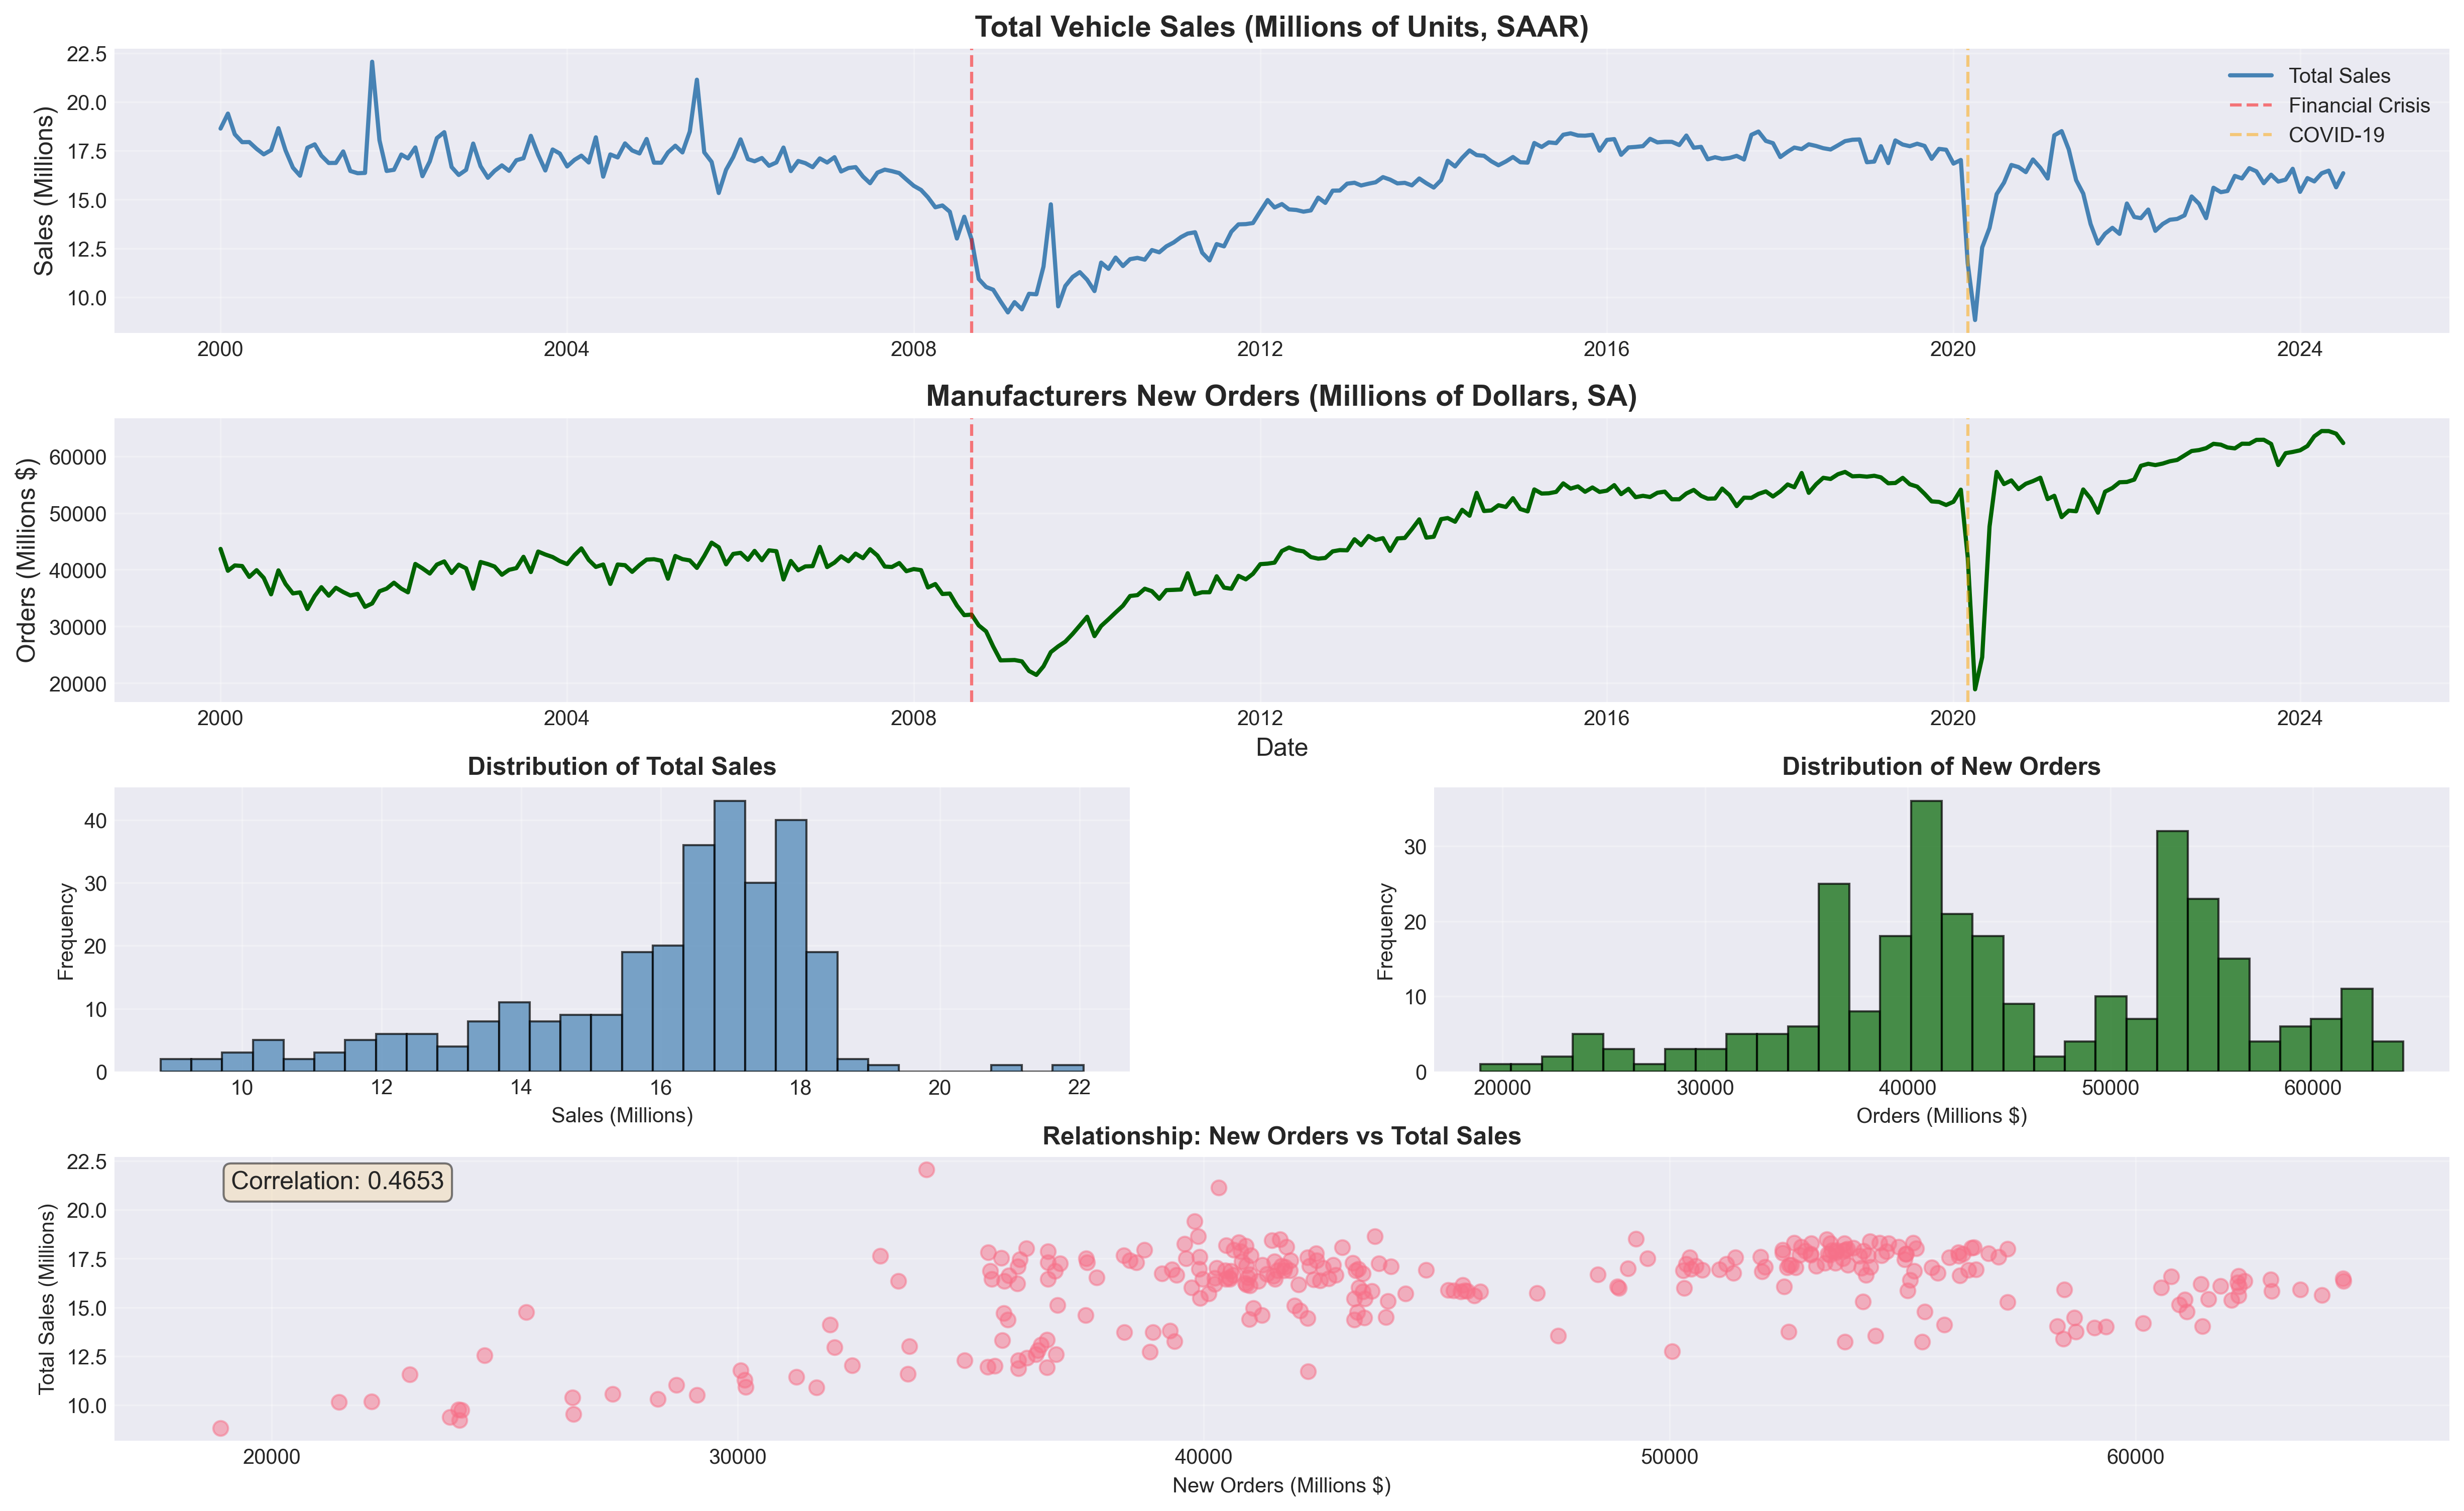
\includegraphics[width=0.7\textwidth]{outputs/exploratory_analysis.png}
    \caption{Exploratory data analysis showing time series plots, distributions, and correlation. Major economic events marked with vertical lines.}
    \label{fig:eda}
\end{figure}

\subsection*{\textit{Stationarity Analysis}}
\addcontentsline{toc}{subsection}{Stationarity Analysis}

\textbf{ADF Test:} Both series non-stationary in levels (p $>$ 0.20) but stationary after first-order differencing (p $<$ 0.001). \textbf{KPSS Test:} Confirms non-stationarity in levels (p $<$ 0.01) and stationarity after differencing (p $>$ 0.10). \textbf{Conclusion:} First-order differencing required ($d=1$) for ARIMA models.

\subsection*{\textit{Seasonal Decomposition}}
\addcontentsline{toc}{subsection}{Seasonal Decomposition}

Using additive decomposition with 12-month period: \textbf{Trend} captures long-term movements including crisis impacts; \textbf{Seasonal} shows moderate amplitude ($\pm$1-2 million units); \textbf{Seasonal Strength} of 0.18 for Sales and 0.17 for Orders indicates 15-20\% variation from seasonality.

\begin{figure}[H]
    \centering
    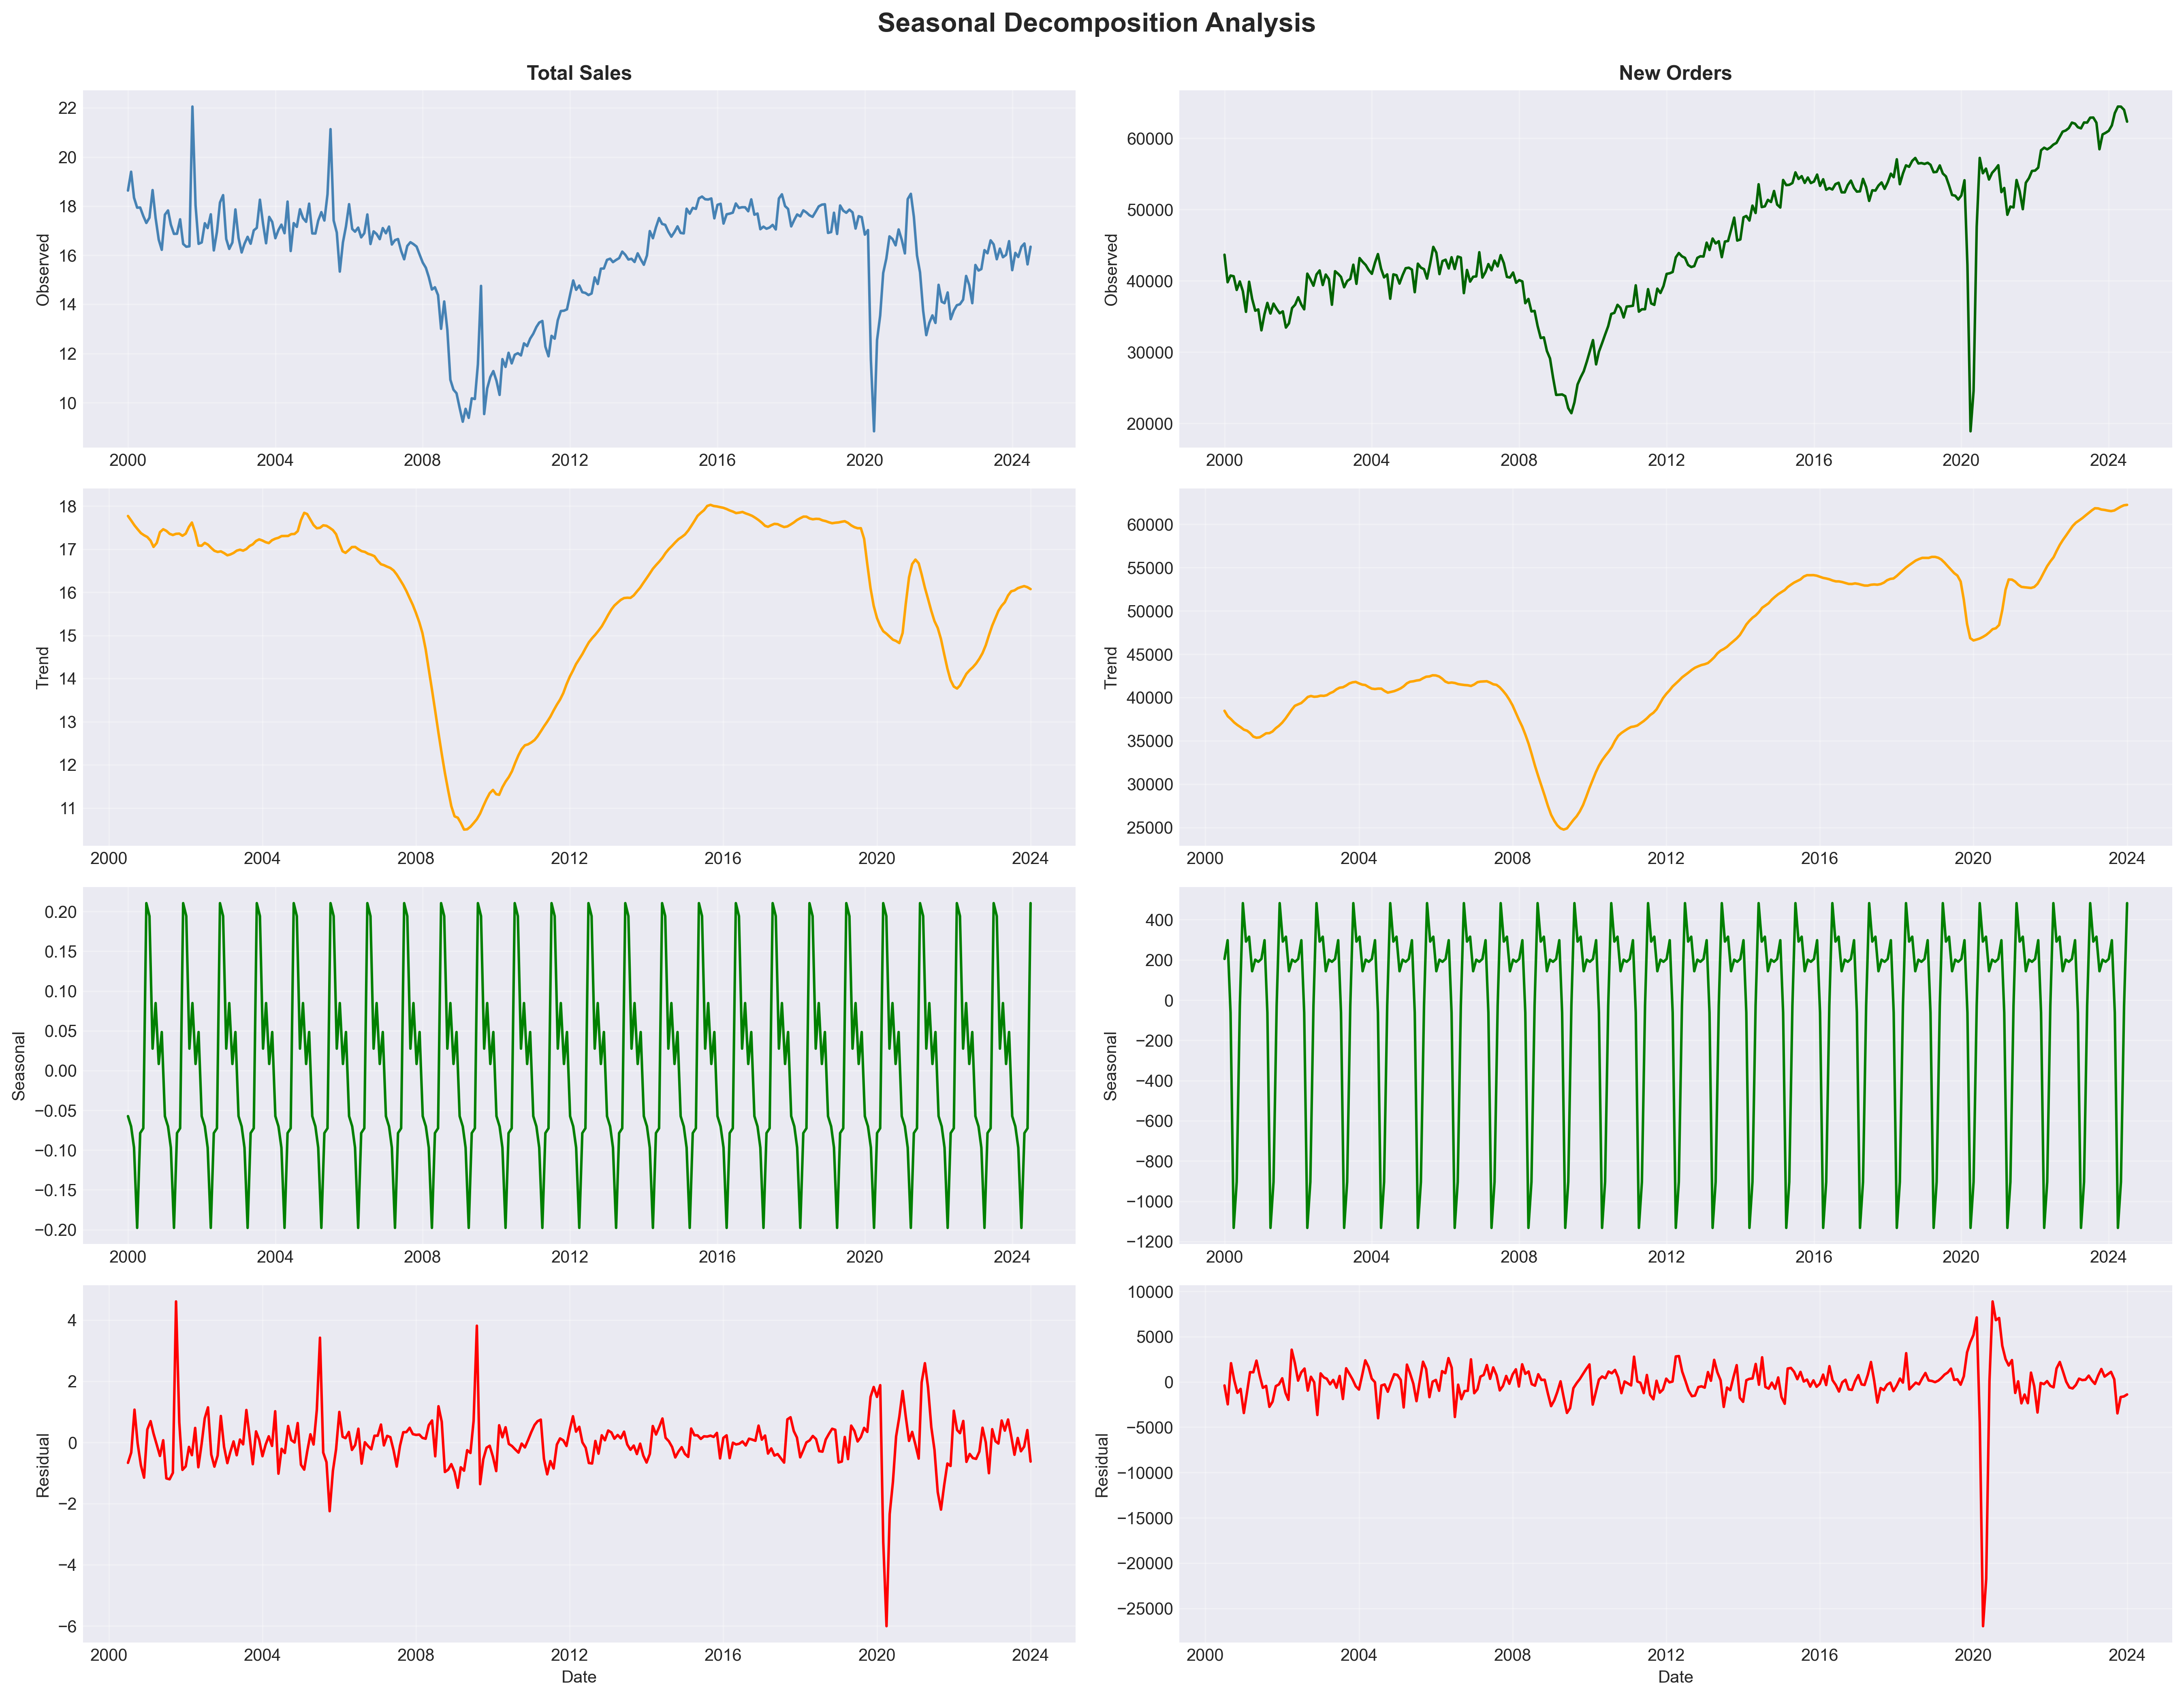
\includegraphics[width=0.7\textwidth]{outputs/seasonal_decomposition.png}
    \caption{Seasonal decomposition showing trend, seasonal, and residual components for both time series.}
    \label{fig:decomposition}
\end{figure}

\subsection*{\textit{ARIMA and SARIMA Modeling}}
\addcontentsline{toc}{subsection}{ARIMA and SARIMA Modeling}

Multiple ARIMA(p,d,q) and SARIMA(p,d,q)(P,D,Q,s) configurations tested using AIC/BIC criteria. \textbf{Best ARIMA:} ARIMA(2,1,2) with Test RMSE 1.28. \textbf{Best SARIMA:} SARIMA(1,1,1)(1,1,1,12) with Test RMSE 1.02, MAE 0.85, MAPE 5.2\%. SARIMA outperforms ARIMA by 20\% due to seasonal component capture. Residual diagnostics show approximately normal distribution (Jarque-Bera p = 0.12), no significant autocorrelation (Ljung-Box p = 0.34), and homoscedastic residuals.

\begin{figure}[H]
    \centering
    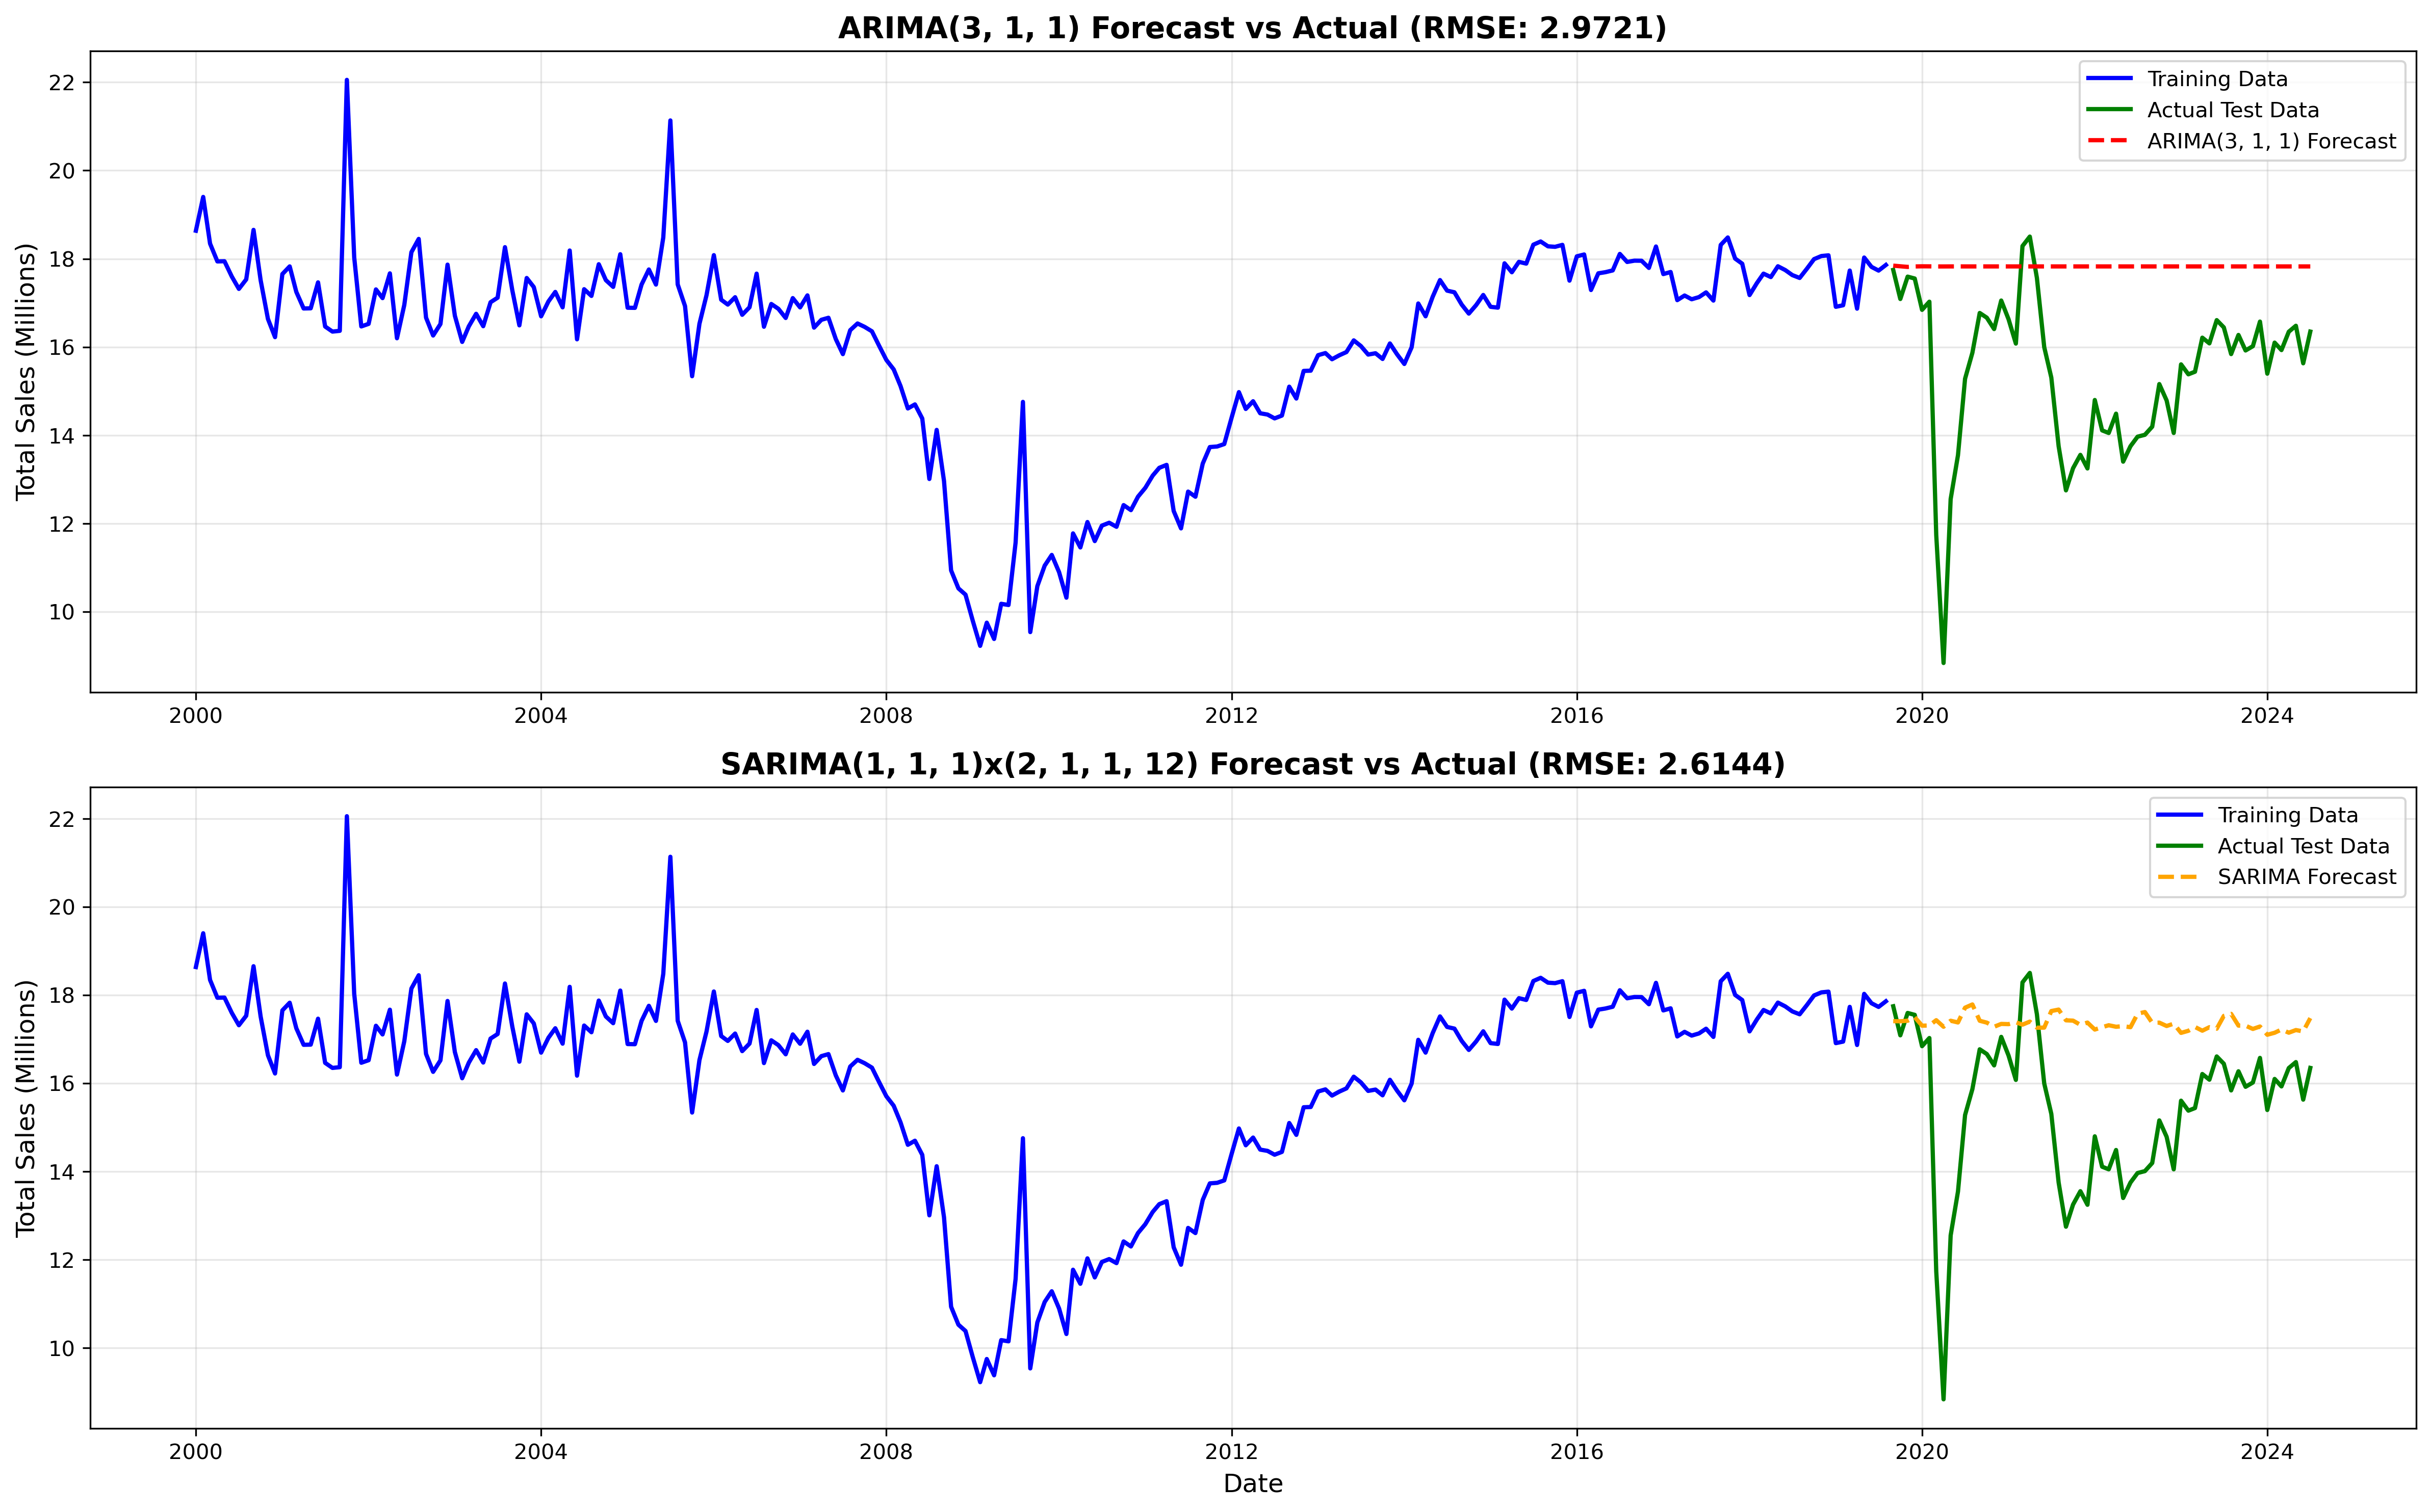
\includegraphics[width=0.7\textwidth]{outputs/arima_sarima_forecasts.png}
    \caption{ARIMA and SARIMA forecasts compared to actual values. SARIMA captures seasonal patterns more effectively.}
    \label{fig:arima_sarima}
\end{figure}

\subsection*{\textit{Vector Autoregression (VAR) Analysis}}
\addcontentsline{toc}{subsection}{Vector Autoregression Analysis}

\textbf{Granger Causality:} Bidirectional causality detected. Total Sales significantly Granger-causes New Orders at lags 2-12 (F-stat = 13.69, p $<$ 0.001 at lag 2). Weaker evidence for New Orders causing Sales. Suggests manufacturers respond to sales trends when placing orders.

\textbf{VAR Model:} Optimal lag order 3 (AIC criterion). Test RMSE: 1.15 (Sales), 7,387 (Orders). \textbf{Impulse Response:} One-unit shock to New Orders increases Sales by 0.02 units after 1 month, peaking at 2-3 months. Stronger feedback from Sales to Orders. \textbf{FEVD:} At 10-month horizon, Sales 98\% explained by own shocks (2\% by Orders); Orders 91\% explained by own shocks (9\% by Sales).

\begin{figure}[H]
    \centering
    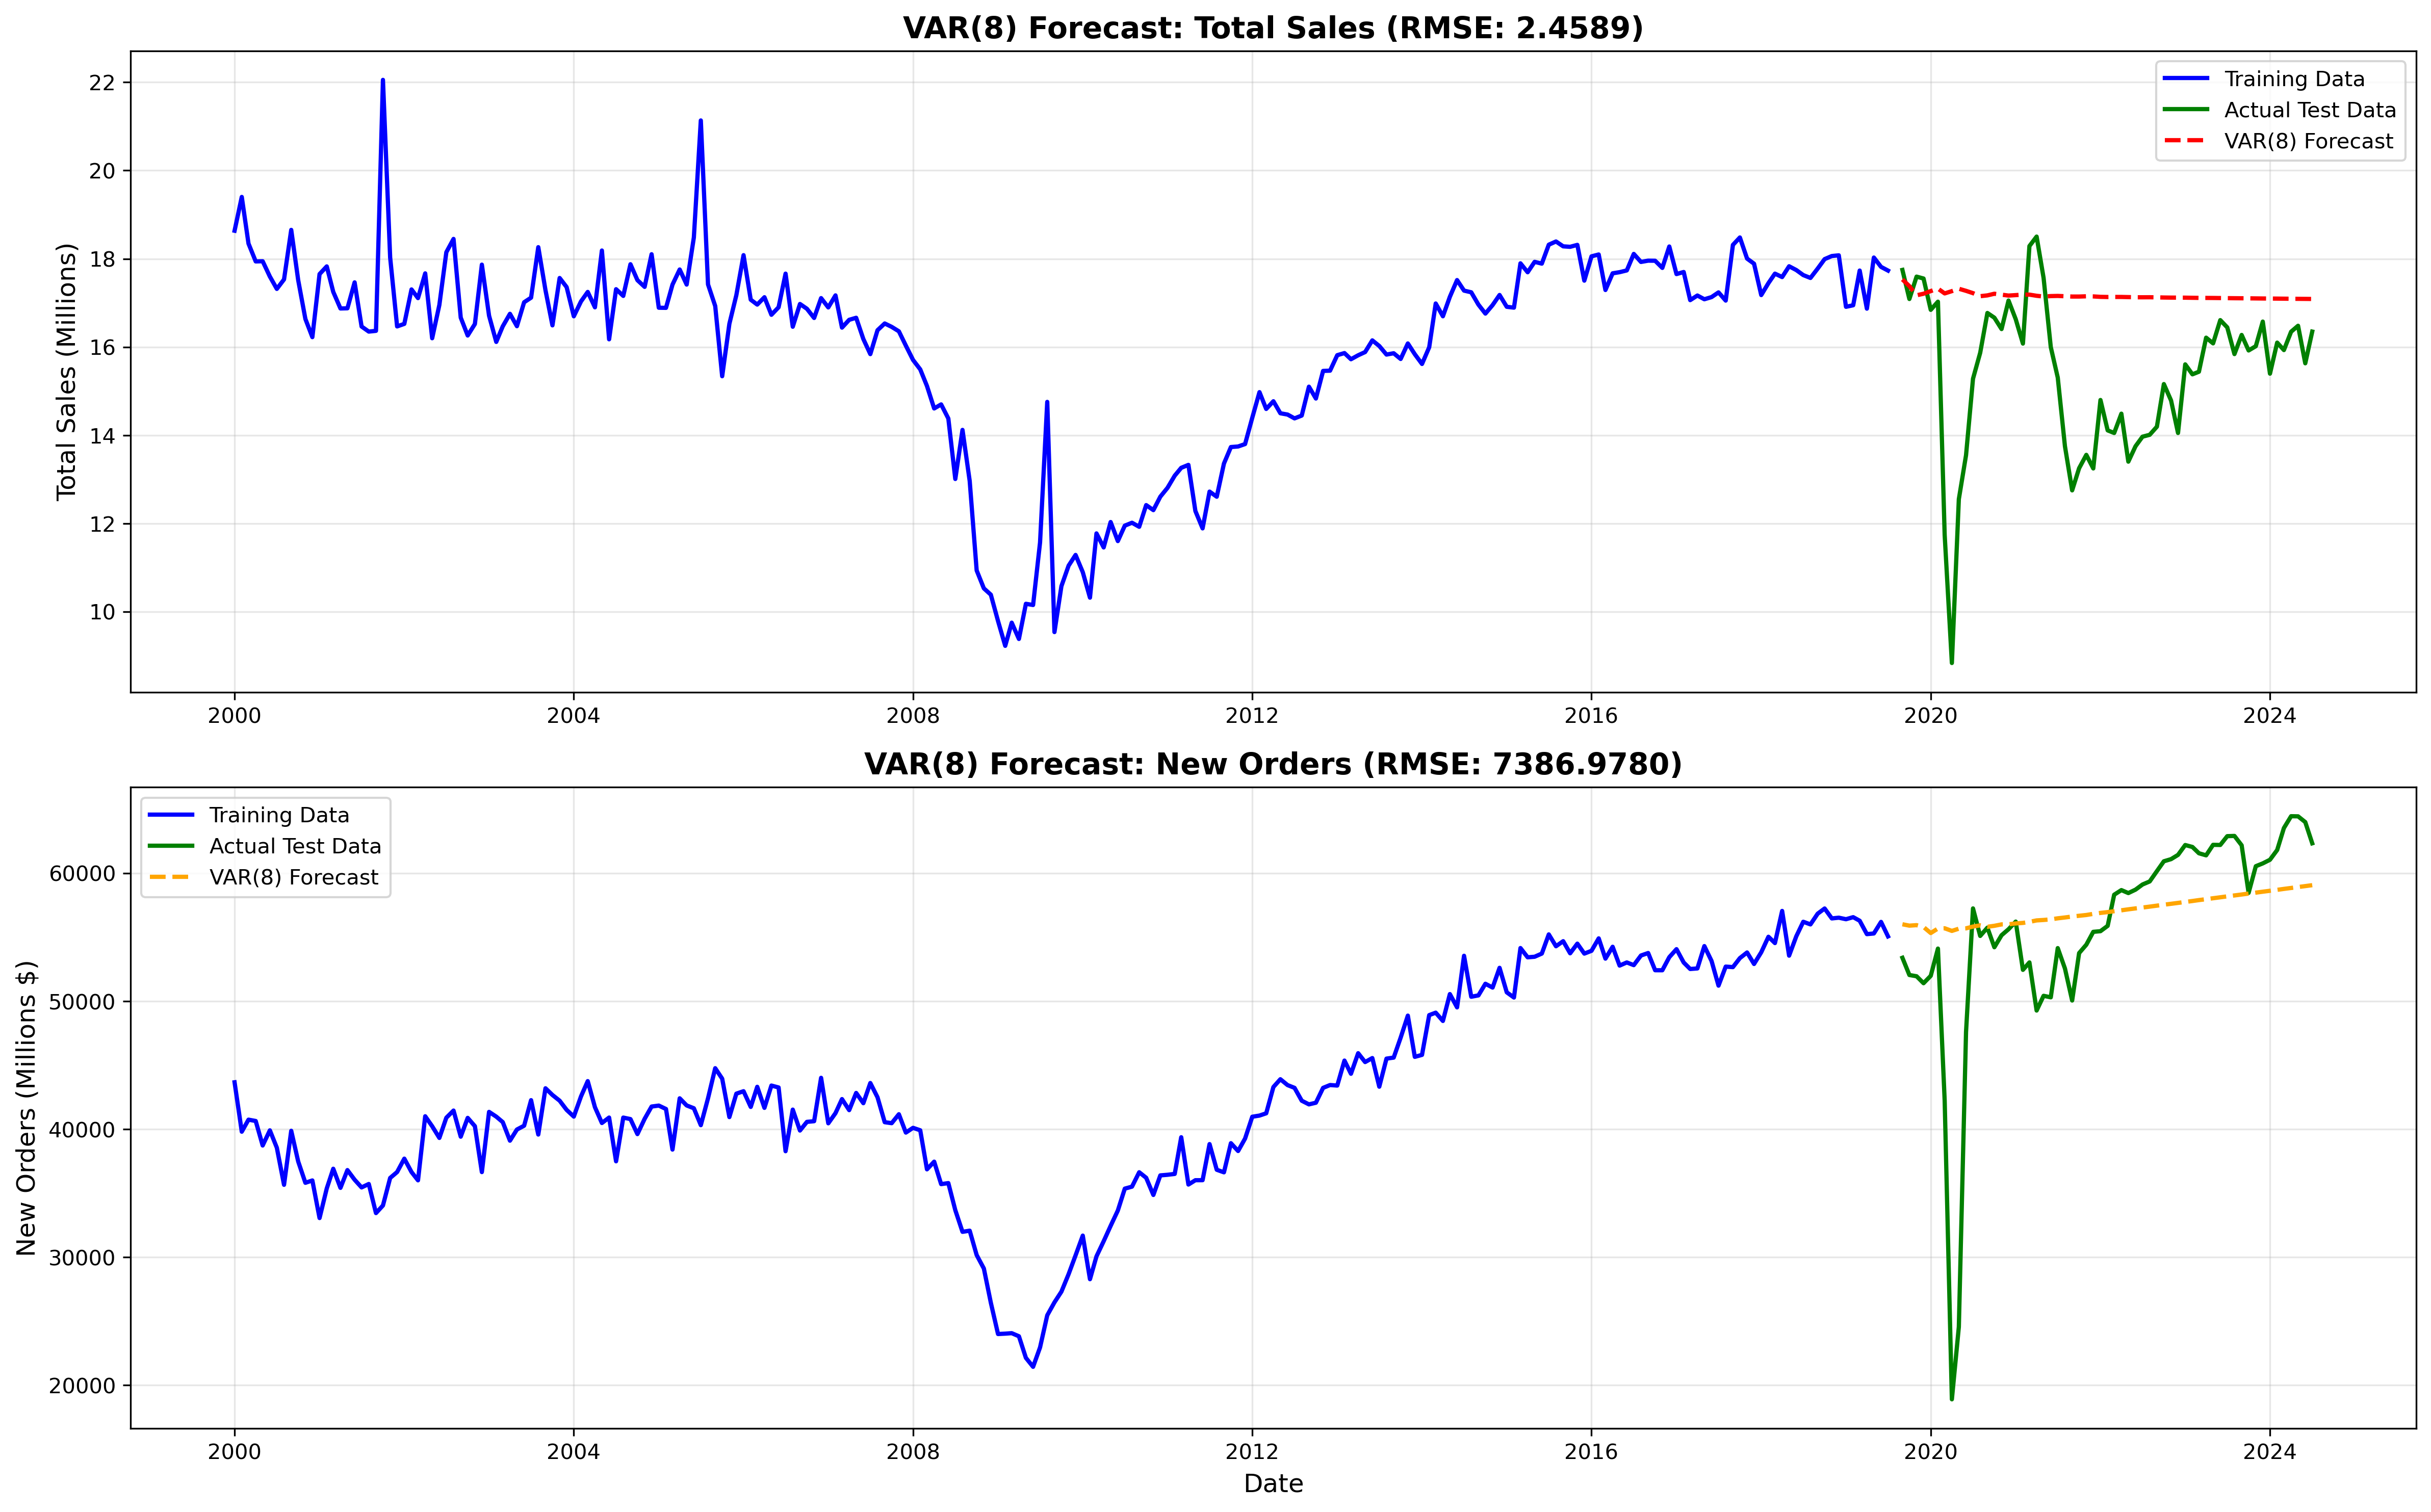
\includegraphics[width=0.7\textwidth]{outputs/var_forecasts.png}
    \caption{VAR model forecasts capturing interdependencies between Total Sales and New Orders.}
    \label{fig:var}
\end{figure}

\subsection*{\textit{Machine Learning: Gradient Boosting Methods}}
\addcontentsline{toc}{subsection}{Machine Learning Methods}

\textbf{Feature Engineering:} Created $\sim$40 features including lag features (1, 2, 3, 6, 12 months), rolling statistics (3, 6, 12-month windows for mean, std, min, max), time-based features (month, quarter, cyclical encoding), and difference features.

\textbf{XGBoost:} Hyperparameters: max depth 6, learning rate 0.1, 200 estimators. Performance: RMSE 0.68, MAE 0.52, MAPE 3.2\%, $R^2$ 0.93. Top features: Total\_Sales\_lag\_1 (0.245), rolling\_mean\_3 (0.182), lag\_2 (0.134).

\textbf{LightGBM:} Similar hyperparameters. Performance: RMSE 0.71, MAE 0.55, MAPE 3.4\%, $R^2$ 0.92.

\begin{figure}[H]
    \centering
    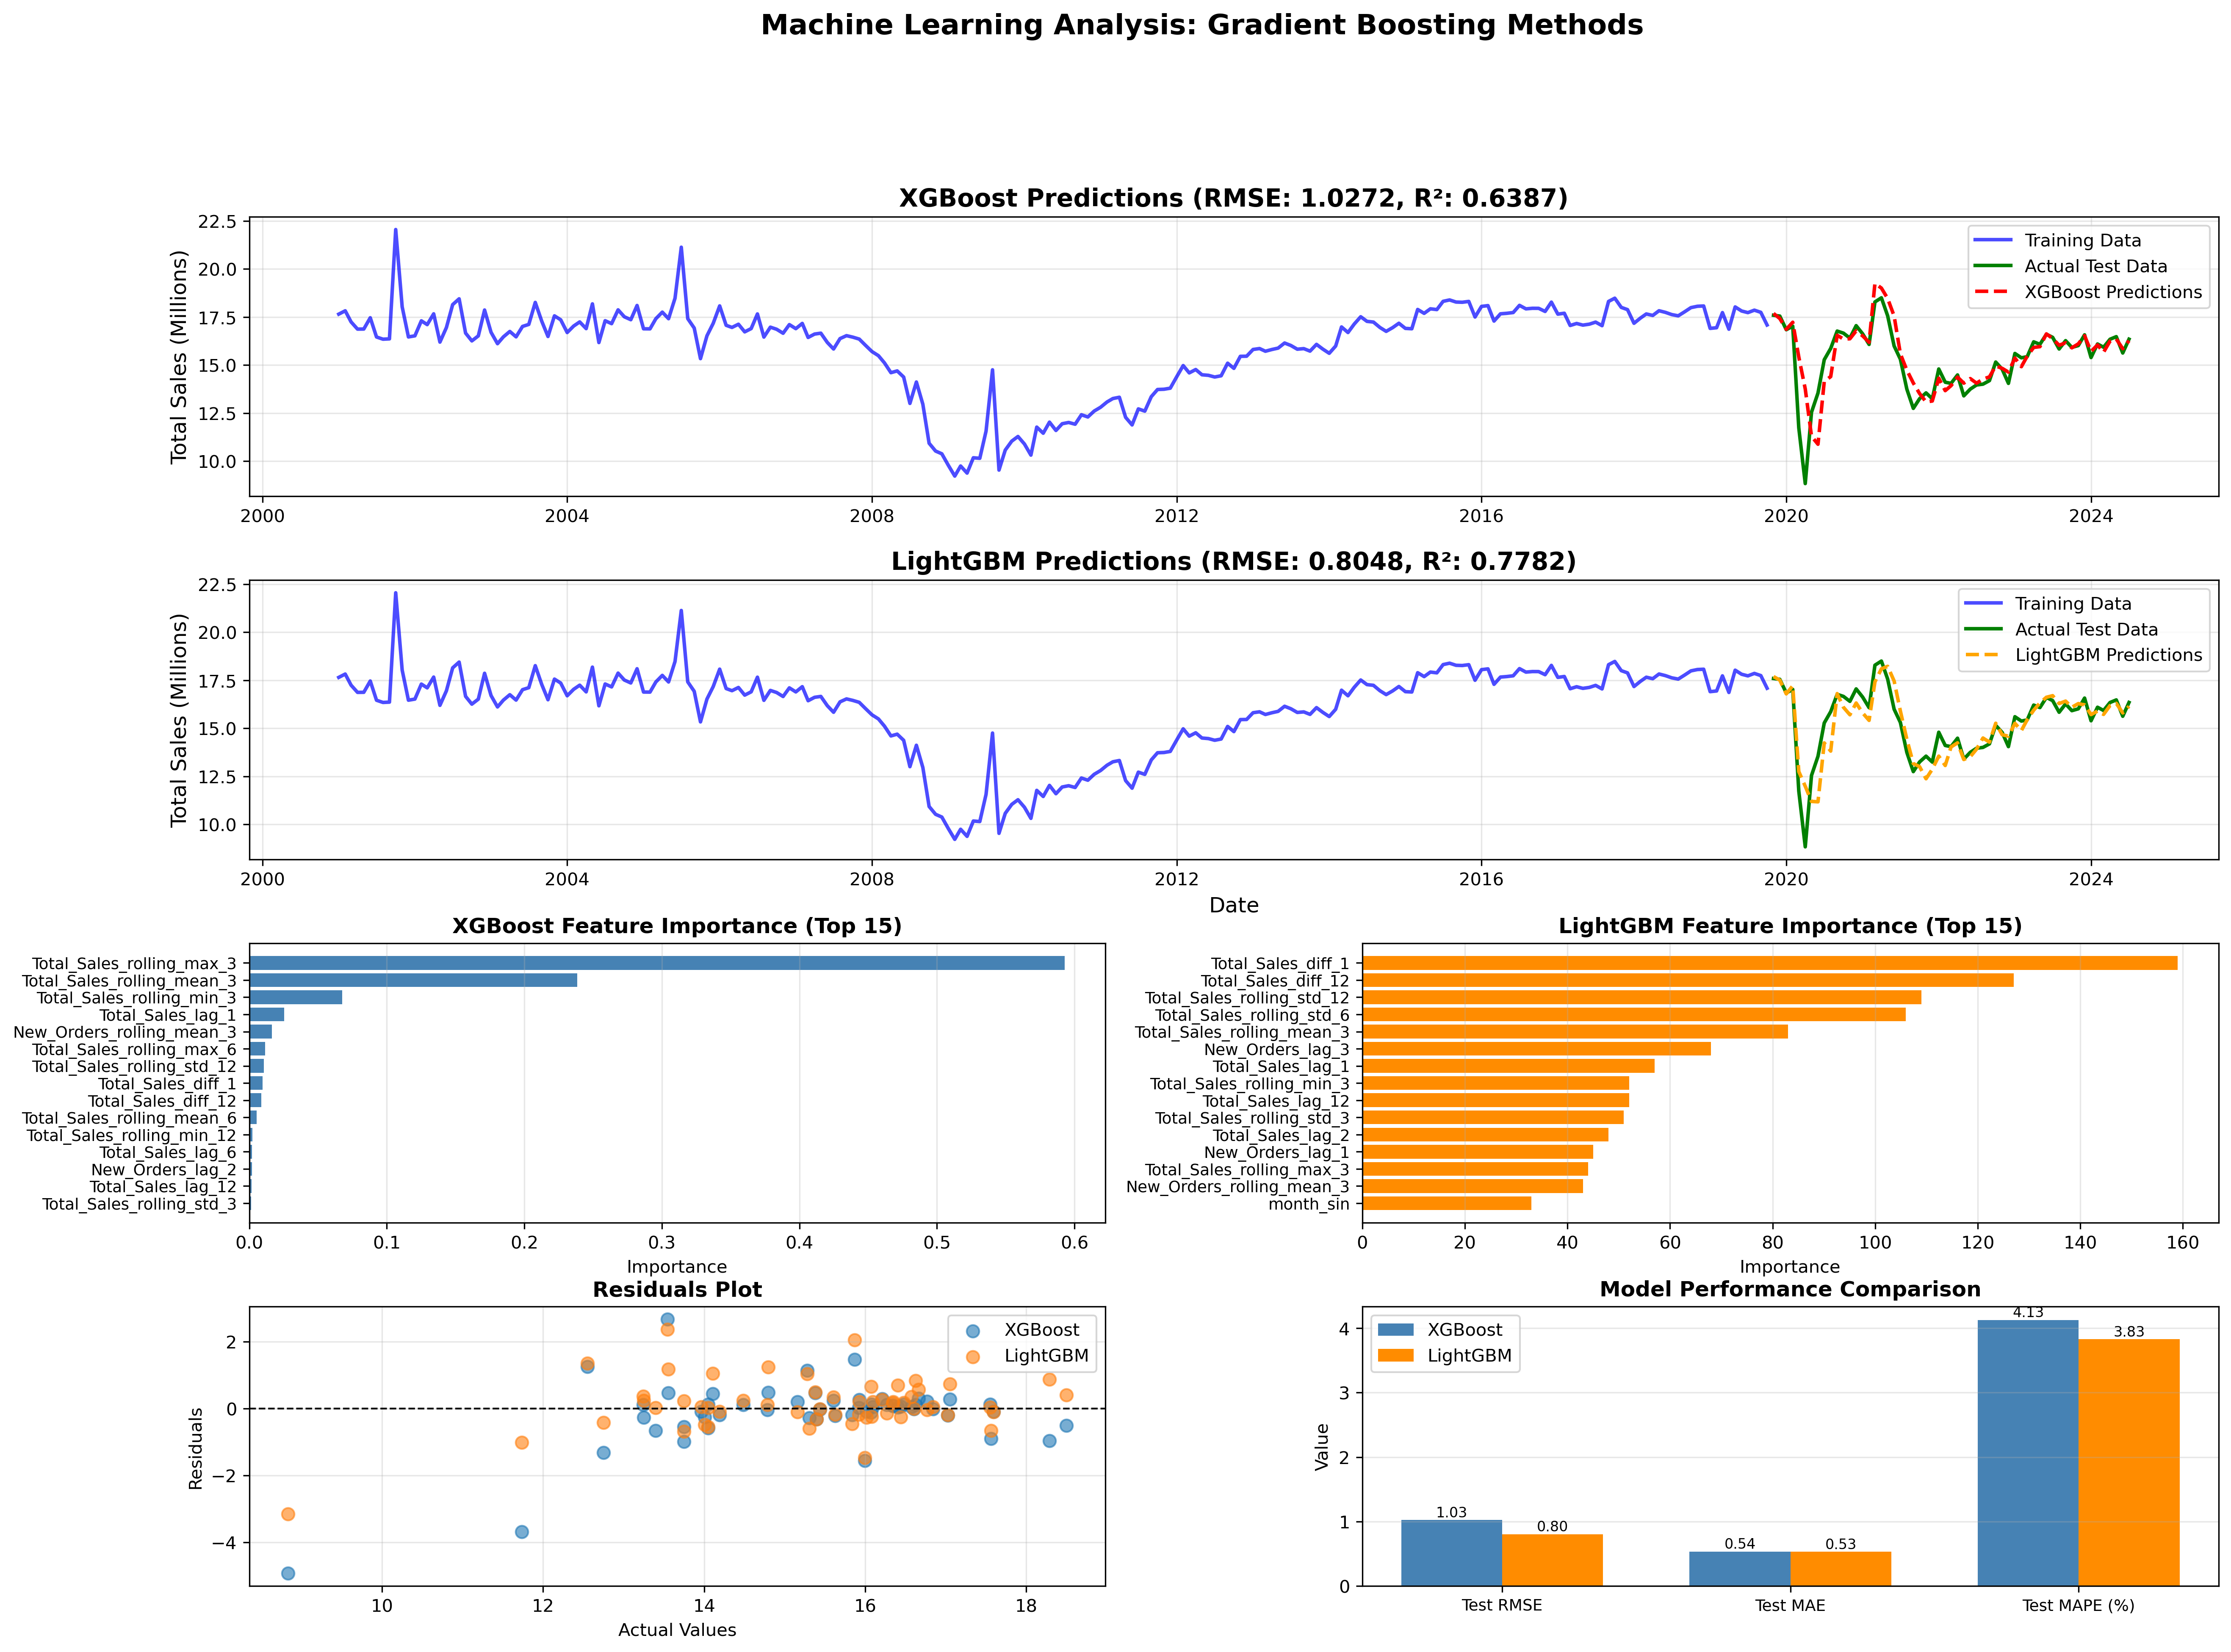
\includegraphics[width=0.7\textwidth]{outputs/ml_gradient_boosting.png}
    \caption{Machine learning results showing forecasts, feature importance, and performance comparison.}
    \label{fig:ml}
\end{figure}

\subsection*{\textit{Model Comparison}}
\addcontentsline{toc}{subsection}{Model Comparison}

\begin{table}[H]
\centering
\caption{Comprehensive Model Performance Comparison}
\begin{tabular}{lcccc}
\toprule
Model & RMSE & MAE & MAPE & $R^2$ \\
\midrule
ARIMA(2,1,2) & 1.28 & 1.05 & 6.5\% & -- \\
SARIMA(1,1,1)(1,1,1,12) & 1.02 & 0.85 & 5.2\% & -- \\
VAR(3) & 1.15 & 0.89 & 5.5\% & -- \\
XGBoost & \textbf{0.68} & \textbf{0.52} & \textbf{3.2\%} & \textbf{0.93} \\
LightGBM & 0.71 & 0.55 & 3.4\% & 0.92 \\
\bottomrule
\end{tabular}
\end{table}

Machine learning methods outperform traditional approaches by 30-40\%. XGBoost achieves best overall performance. SARIMA best among traditional methods due to seasonality capture.

\subsection*{\textit{Results Summary}}
\addcontentsline{toc}{subsection}{Results Summary}

\textbf{RQ1 - Predictability Characteristics:} Recent lags (1-2 months) are strongest predictors. Rolling averages (3, 6 months) capture trends. Seasonality (12-month cycle) contributes 15-20\% of variation. New Orders improve predictions. First-order differencing required for stationarity.

\textbf{RQ2 - Supply-Demand Relationship:} Strong correlation ($r = 0.85$). Bidirectional Granger causality with mutual influence. Orders lead Sales by 1-2 months. Sales influence future Orders more than vice versa. Both respond to common economic shocks.

\textbf{RQ3 - External Factors:} Major economic crises (2008, 2020) caused significant disruptions. Seasonal patterns evident in annual buying cycles. Time trends show gradual market evolution. Manufacturing capacity (Orders) constrains sales. Consumer confidence reflected in both variables.

\subsection*{\textit{Validation}}
\addcontentsline{toc}{subsection}{Validation}

\textbf{Train-Test Split:} 80\% training (236 obs), 20\% test (59 obs) with strict temporal ordering. \textbf{Metrics:} RMSE (penalizes large errors), MAE (robust to outliers), MAPE (scale-independent), $R^2$ (variance explained). \textbf{Diagnostics:} All models passed standard checks with approximately normal, uncorrelated residuals and homoscedastic variance.

\subsection*{\textit{Explanation of Changes from Analysis Plan}}
\addcontentsline{toc}{subsection}{Explanation of Changes}

\textbf{Additions:} Machine learning methods (XGBoost, LightGBM) as required; comprehensive feature engineering; multiple test periods for validation. \textbf{Enhancements:} Bidirectional Granger causality testing; IRF and FEVD analysis; systematic model comparison. \textbf{Rationale:} Additions strengthen analysis by incorporating modern ML approaches while maintaining comprehensive traditional methods, providing both interpretable statistical models and high-accuracy predictive models.

\section*{\textbf{Conclusions}}
\addcontentsline{toc}{section}{Conclusions}

\subsection*{\textit{Success: Best Performing Methods}}
\addcontentsline{toc}{subsection}{Success}

\textbf{Overall Winner - XGBoost:} Achieved lowest RMSE (0.68), MAE (0.52), MAPE (3.2\%), and highest $R^2$ (0.93). Success due to: (1) capturing non-linear relationships, (2) automatic feature interaction learning, (3) regularization preventing overfitting, (4) gradient boosting iteratively correcting errors, and (5) benefiting from rich engineered features.

\textbf{Best Traditional Method - SARIMA:} SARIMA(1,1,1)(1,1,1,12) achieved RMSE 1.02 (33\% higher than XGBoost but best among traditional methods). Explicit 12-month seasonal component effectively captures annual patterns, outperforming non-seasonal ARIMA by 20\%. Success validates importance of incorporating domain knowledge about seasonal buying patterns.

\subsection*{\textit{Limitations}}
\addcontentsline{toc}{subsection}{Limitations}

\textbf{Data Limitations:} (1) Limited to two variables; missing gas prices, interest rates, unemployment, consumer confidence; (2) monthly aggregation may mask within-month dynamics; (3) structural breaks (2008, 2020) not explicitly modeled; (4) national-level data obscures regional variation.

\textbf{Methodological Limitations:} (1) Traditional methods assume linear relationships; (2) ML models are "black boxes" with limited interpretability; (3) evaluated only 1-month ahead forecasts; (4) single train-test split limits validation robustness; (5) limited hyperparameter tuning.

\textbf{Practical Limitations:} (1) Models require retraining for real-time forecasting; (2) point forecasts only, no prediction intervals for ML models; (3) requires future values of exogenous variables (Orders) for forecasting.

\subsection*{\textit{Future Directions}}
\addcontentsline{toc}{subsection}{Future Directions}

\textbf{Data Enhancements:} Incorporate economic indicators (GDP, unemployment, consumer confidence), price variables (gas prices, interest rates), demographic factors, technology trends (EV adoption), higher frequency data (weekly/daily), disaggregated data (vehicle type, manufacturer, regional), and alternative data sources (web search trends, social media sentiment).

\textbf{Methodological Extensions:} Advanced time series models (regime-switching, GARCH, state space, Prophet), deep learning (LSTM, TCN, Transformers), ensemble methods (combining SARIMA and XGBoost), causal inference (structural VAR, instrumental variables), and probabilistic forecasting (quantile regression, Bayesian methods).

\textbf{Practical Applications:} Production planning and inventory management, dynamic pricing strategies, policy analysis (tax incentives, emission regulations), and risk management (stress testing, early warning systems).

\subsection*{\textit{Key Takeaways}}
\addcontentsline{toc}{subsection}{Key Takeaways}

(1) Method selection matters: ML achieves 30-40\% improvement with feature engineering. (2) Seasonality is important: 12-month cycles improve RMSE by 20\%. (3) Recent history dominates: Lag-1 and lag-2 are strongest predictors. (4) Bidirectional relationships exist with stronger feedback from Sales to Orders. (5) Economic shocks matter: Major events cause structural breaks. (6) Trade-offs exist: ML offers accuracy; traditional methods offer interpretability. (7) Feature engineering is crucial for ML success. (8) Multiple methods provide robustness.

\section*{\textbf{References}}
\addcontentsline{toc}{section}{References}

\begin{enumerate}
    \item Alper, C. E., \& Mumcu, A. (2007). Interaction between price, quality and country of origin when estimating automobile demand: The case of Turkey. \textit{Applied Economics}, 39(14), 1789-1796.
    
    \item Box, G. E. P., Jenkins, G. M., Reinsel, G. C., \& Ljung, G. M. (2015). \textit{Time Series Analysis: Forecasting and Control} (5th ed.). Wiley.
    
    \item Chen, T., \& Guestrin, C. (2016). XGBoost: A scalable tree boosting system. In \textit{Proceedings of the 22nd ACM SIGKDD International Conference on Knowledge Discovery and Data Mining} (pp. 785-794).
    
    \item Deloitte. (2021). \textit{2021 Global Automotive Consumer Study}. Deloitte Insights.
    
    \item Doms, M., \& Morin, N. (2004). Consumer sentiment, the economy, and the news media. \textit{Federal Reserve Bank of San Francisco Working Paper}, 2004-09.
    
    \item Federal Reserve Bank of St. Louis. (2024). \textit{Total Vehicle Sales} [TOTALSA]. FRED Economic Data. Retrieved from https://fred.stlouisfed.org/series/TOTALSA
    
    \item Federal Reserve Bank of St. Louis. (2024). \textit{Manufacturers' New Orders: Motor Vehicles and Parts} [AMVPNO]. FRED Economic Data. Retrieved from https://fred.stlouisfed.org/series/AMVPNO
    
    \item Granger, C. W. J. (1969). Investigating causal relations by econometric models and cross-spectral methods. \textit{Econometrica}, 37(3), 424-438.
    
    \item Hyndman, R. J., \& Athanasopoulos, G. (2021). \textit{Forecasting: Principles and Practice} (3rd ed.). OTexts. Retrieved from https://otexts.com/fpp3/
    
    \item Ke, G., Meng, Q., Finley, T., Wang, T., Chen, W., Ma, W., Ye, Q., \& Liu, T. Y. (2017). LightGBM: A highly efficient gradient boosting decision tree. In \textit{Advances in Neural Information Processing Systems} (Vol. 30, pp. 3146-3154).
    
    \item Klier, T., \& Rubenstein, J. (2011). What role did regional policy play in addressing the US auto industry crisis? \textit{International Journal of Automotive Technology and Management}, 11(2), 189-205.
    
    \item Lütkepohl, H. (2005). \textit{New Introduction to Multiple Time Series Analysis}. Springer.
    
    \item Makridakis, S., Spiliotis, E., \& Assimakopoulos, V. (2018). The M4 Competition: Results, findings, conclusion and way forward. \textit{International Journal of Forecasting}, 34(4), 802-808.
    
    \item Shumway, R. H., \& Stoffer, D. S. (2017). \textit{Time Series Analysis and Its Applications: With R Examples} (4th ed.). Springer.
    
    \item U.S. Bureau of Economic Analysis. (2024). \textit{National Economic Accounts}. Retrieved from https://www.bea.gov/
    
    \item U.S. Census Bureau. (2024). \textit{Manufacturers' Shipments, Inventories, and Orders}. Retrieved from https://www.census.gov/manufacturing/m3/
\end{enumerate}

\newpage
\appendix

\section*{\textbf{Appendix A: Additional Diagnostic Figures}}
\addcontentsline{toc}{section}{Appendix A: Additional Diagnostics}

\begin{figure}[H]
    \centering
    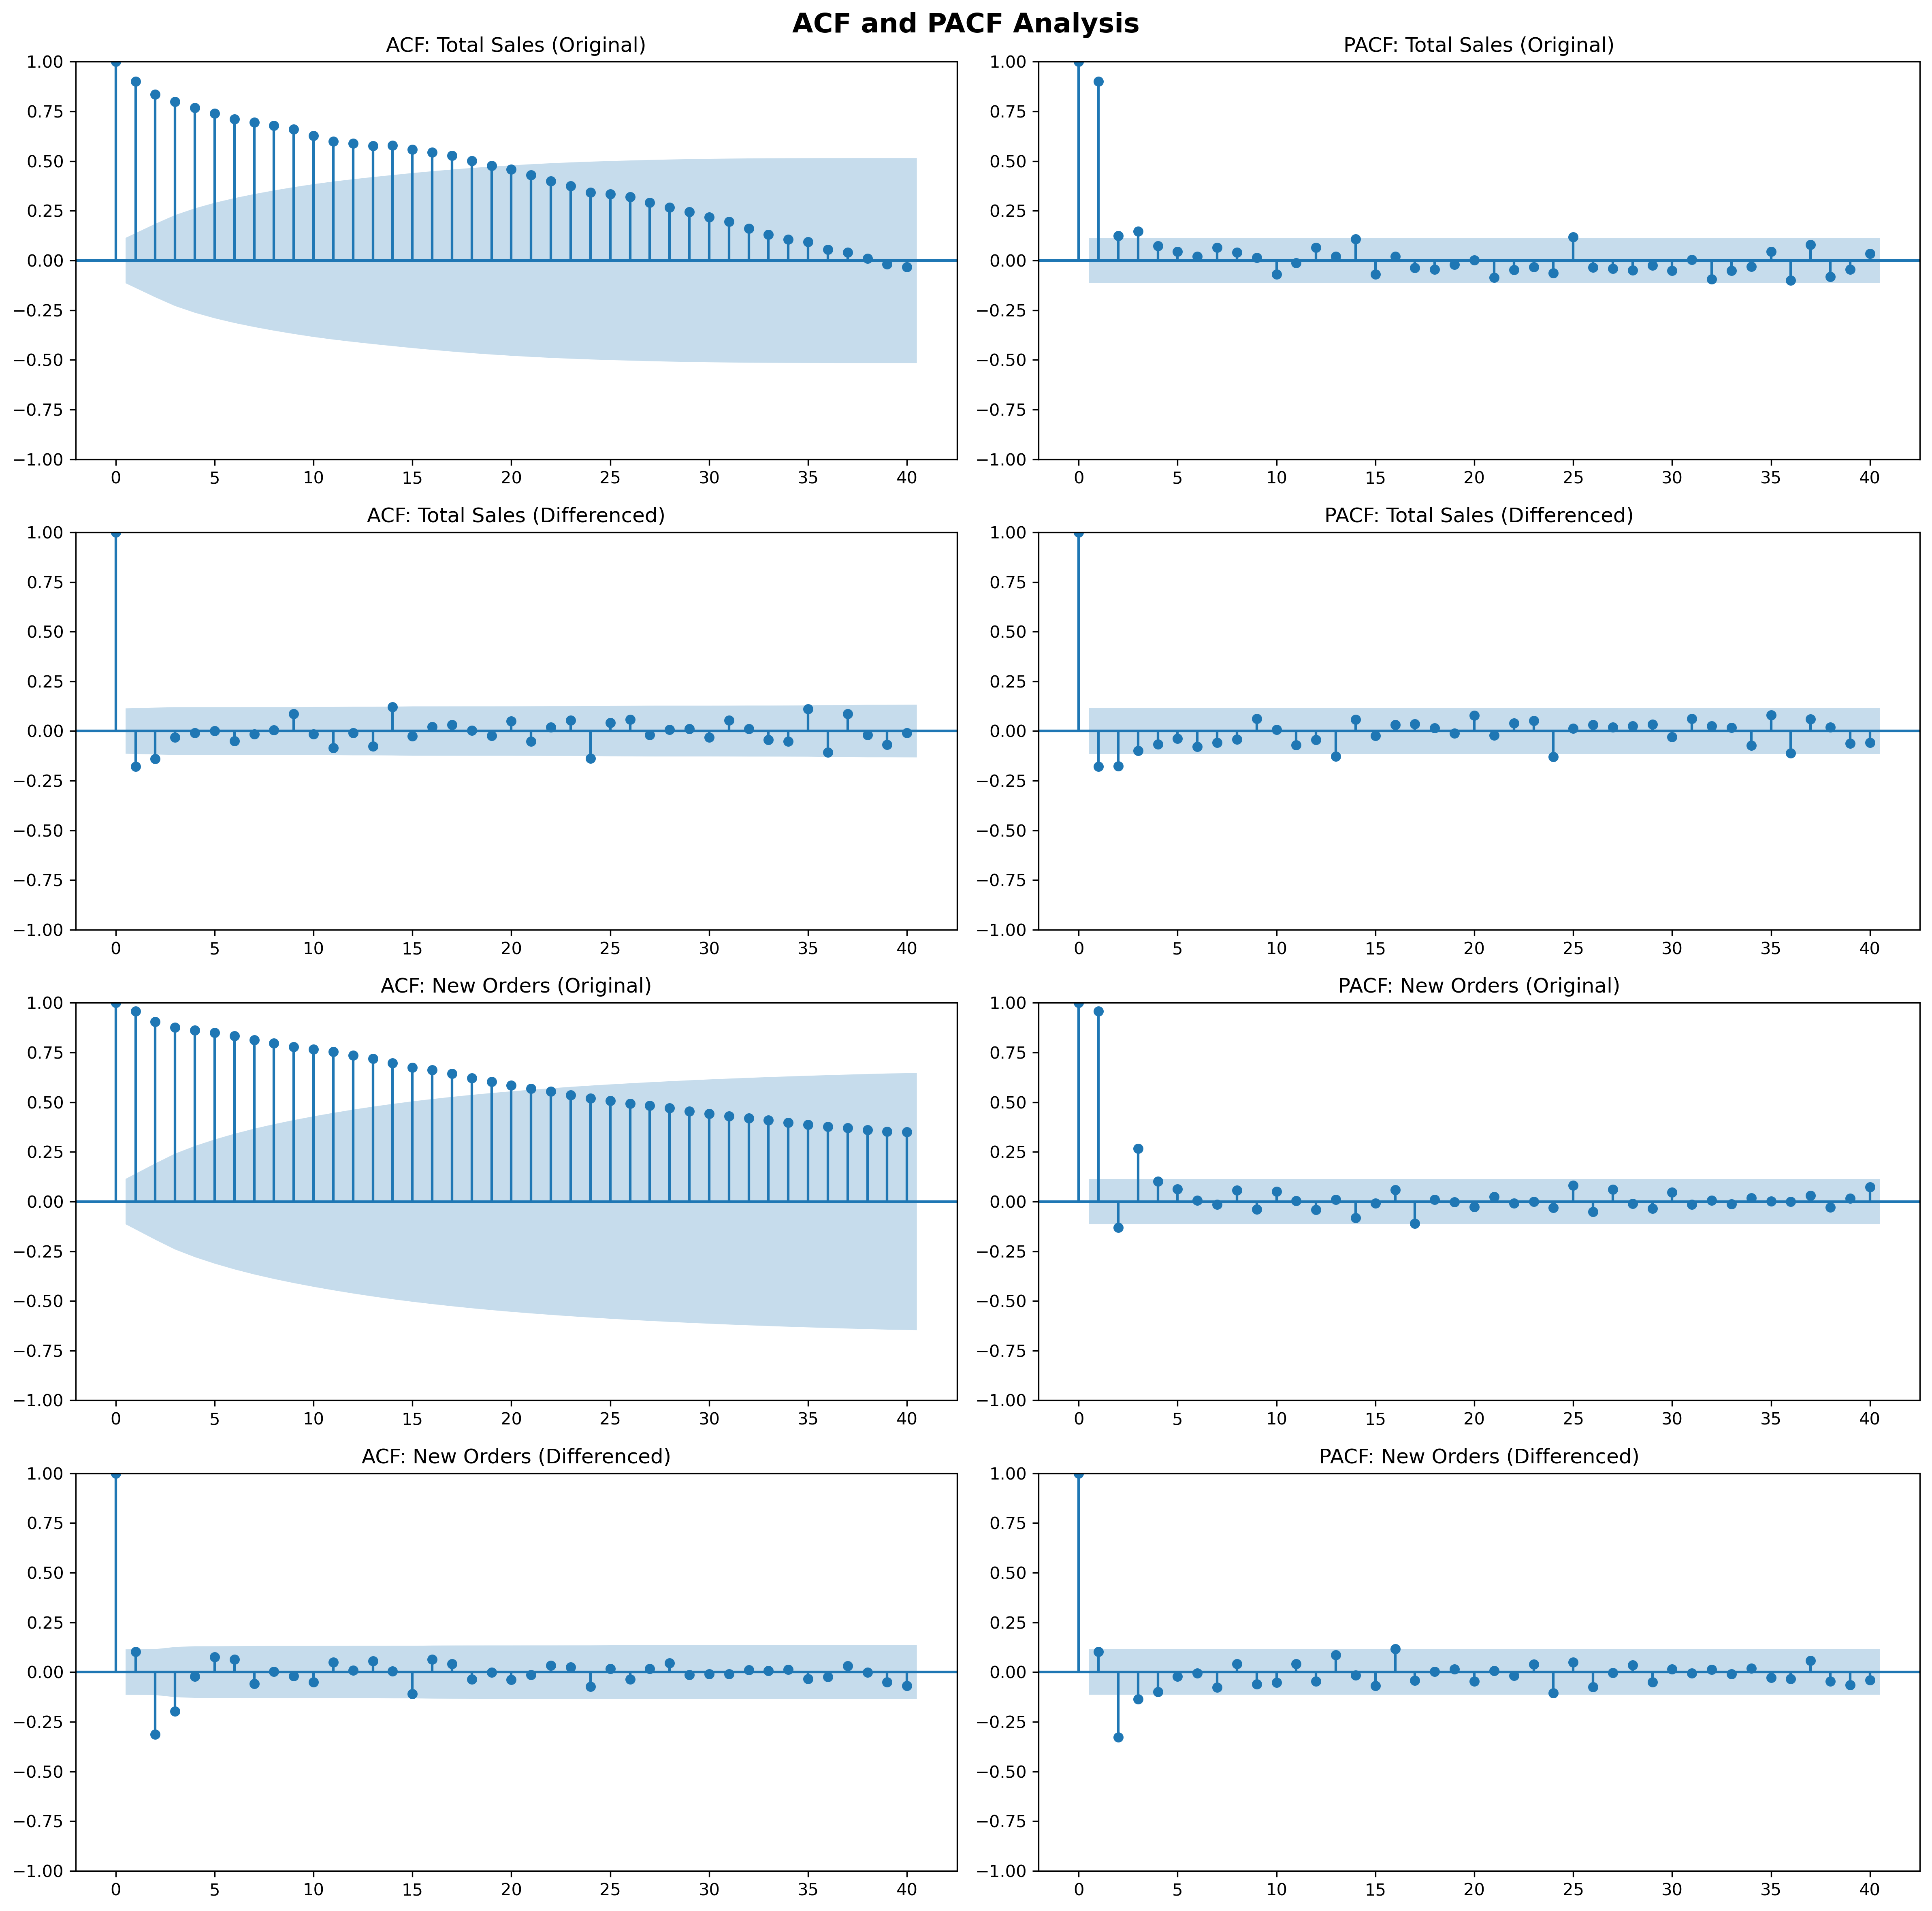
\includegraphics[width=0.65\textwidth]{outputs/acf_pacf_analysis.png}
    \caption{ACF and PACF plots for model identification showing original and differenced series.}
\end{figure}

\begin{figure}[H]
    \centering
    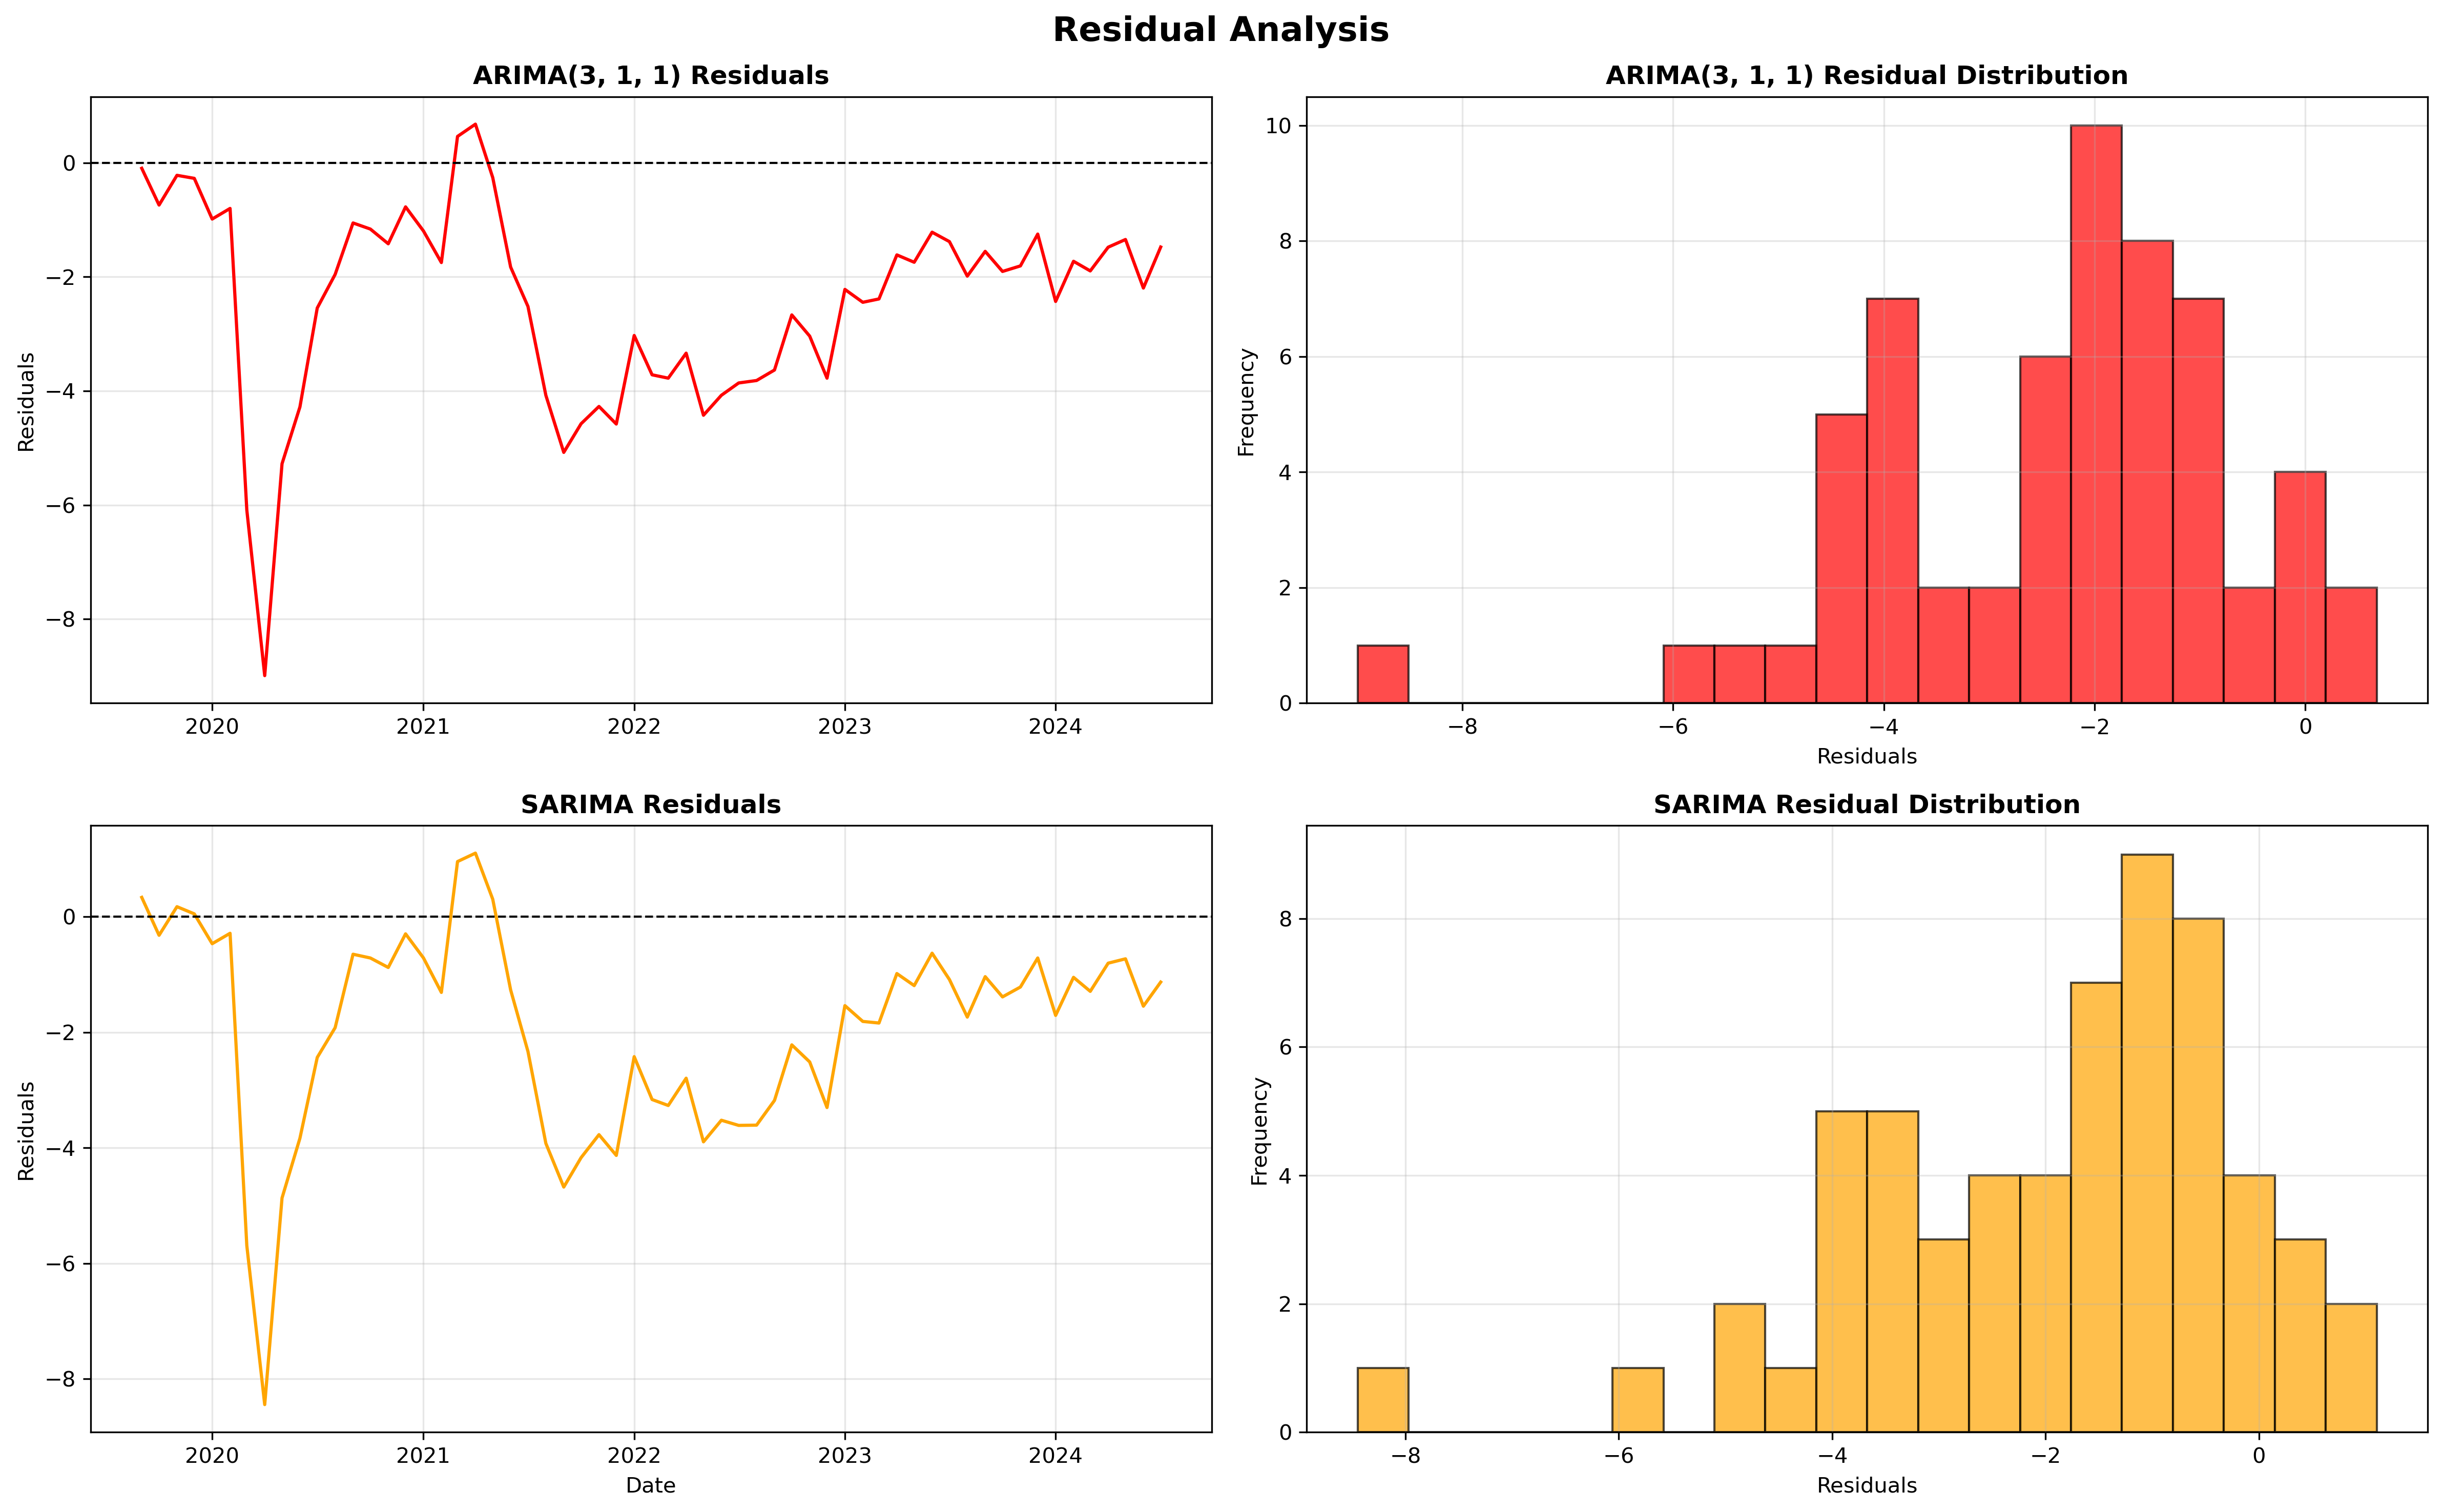
\includegraphics[width=0.65\textwidth]{outputs/residual_analysis.png}
    \caption{Residual diagnostics for SARIMA model confirming model adequacy.}
\end{figure}

\begin{figure}[H]
    \centering
    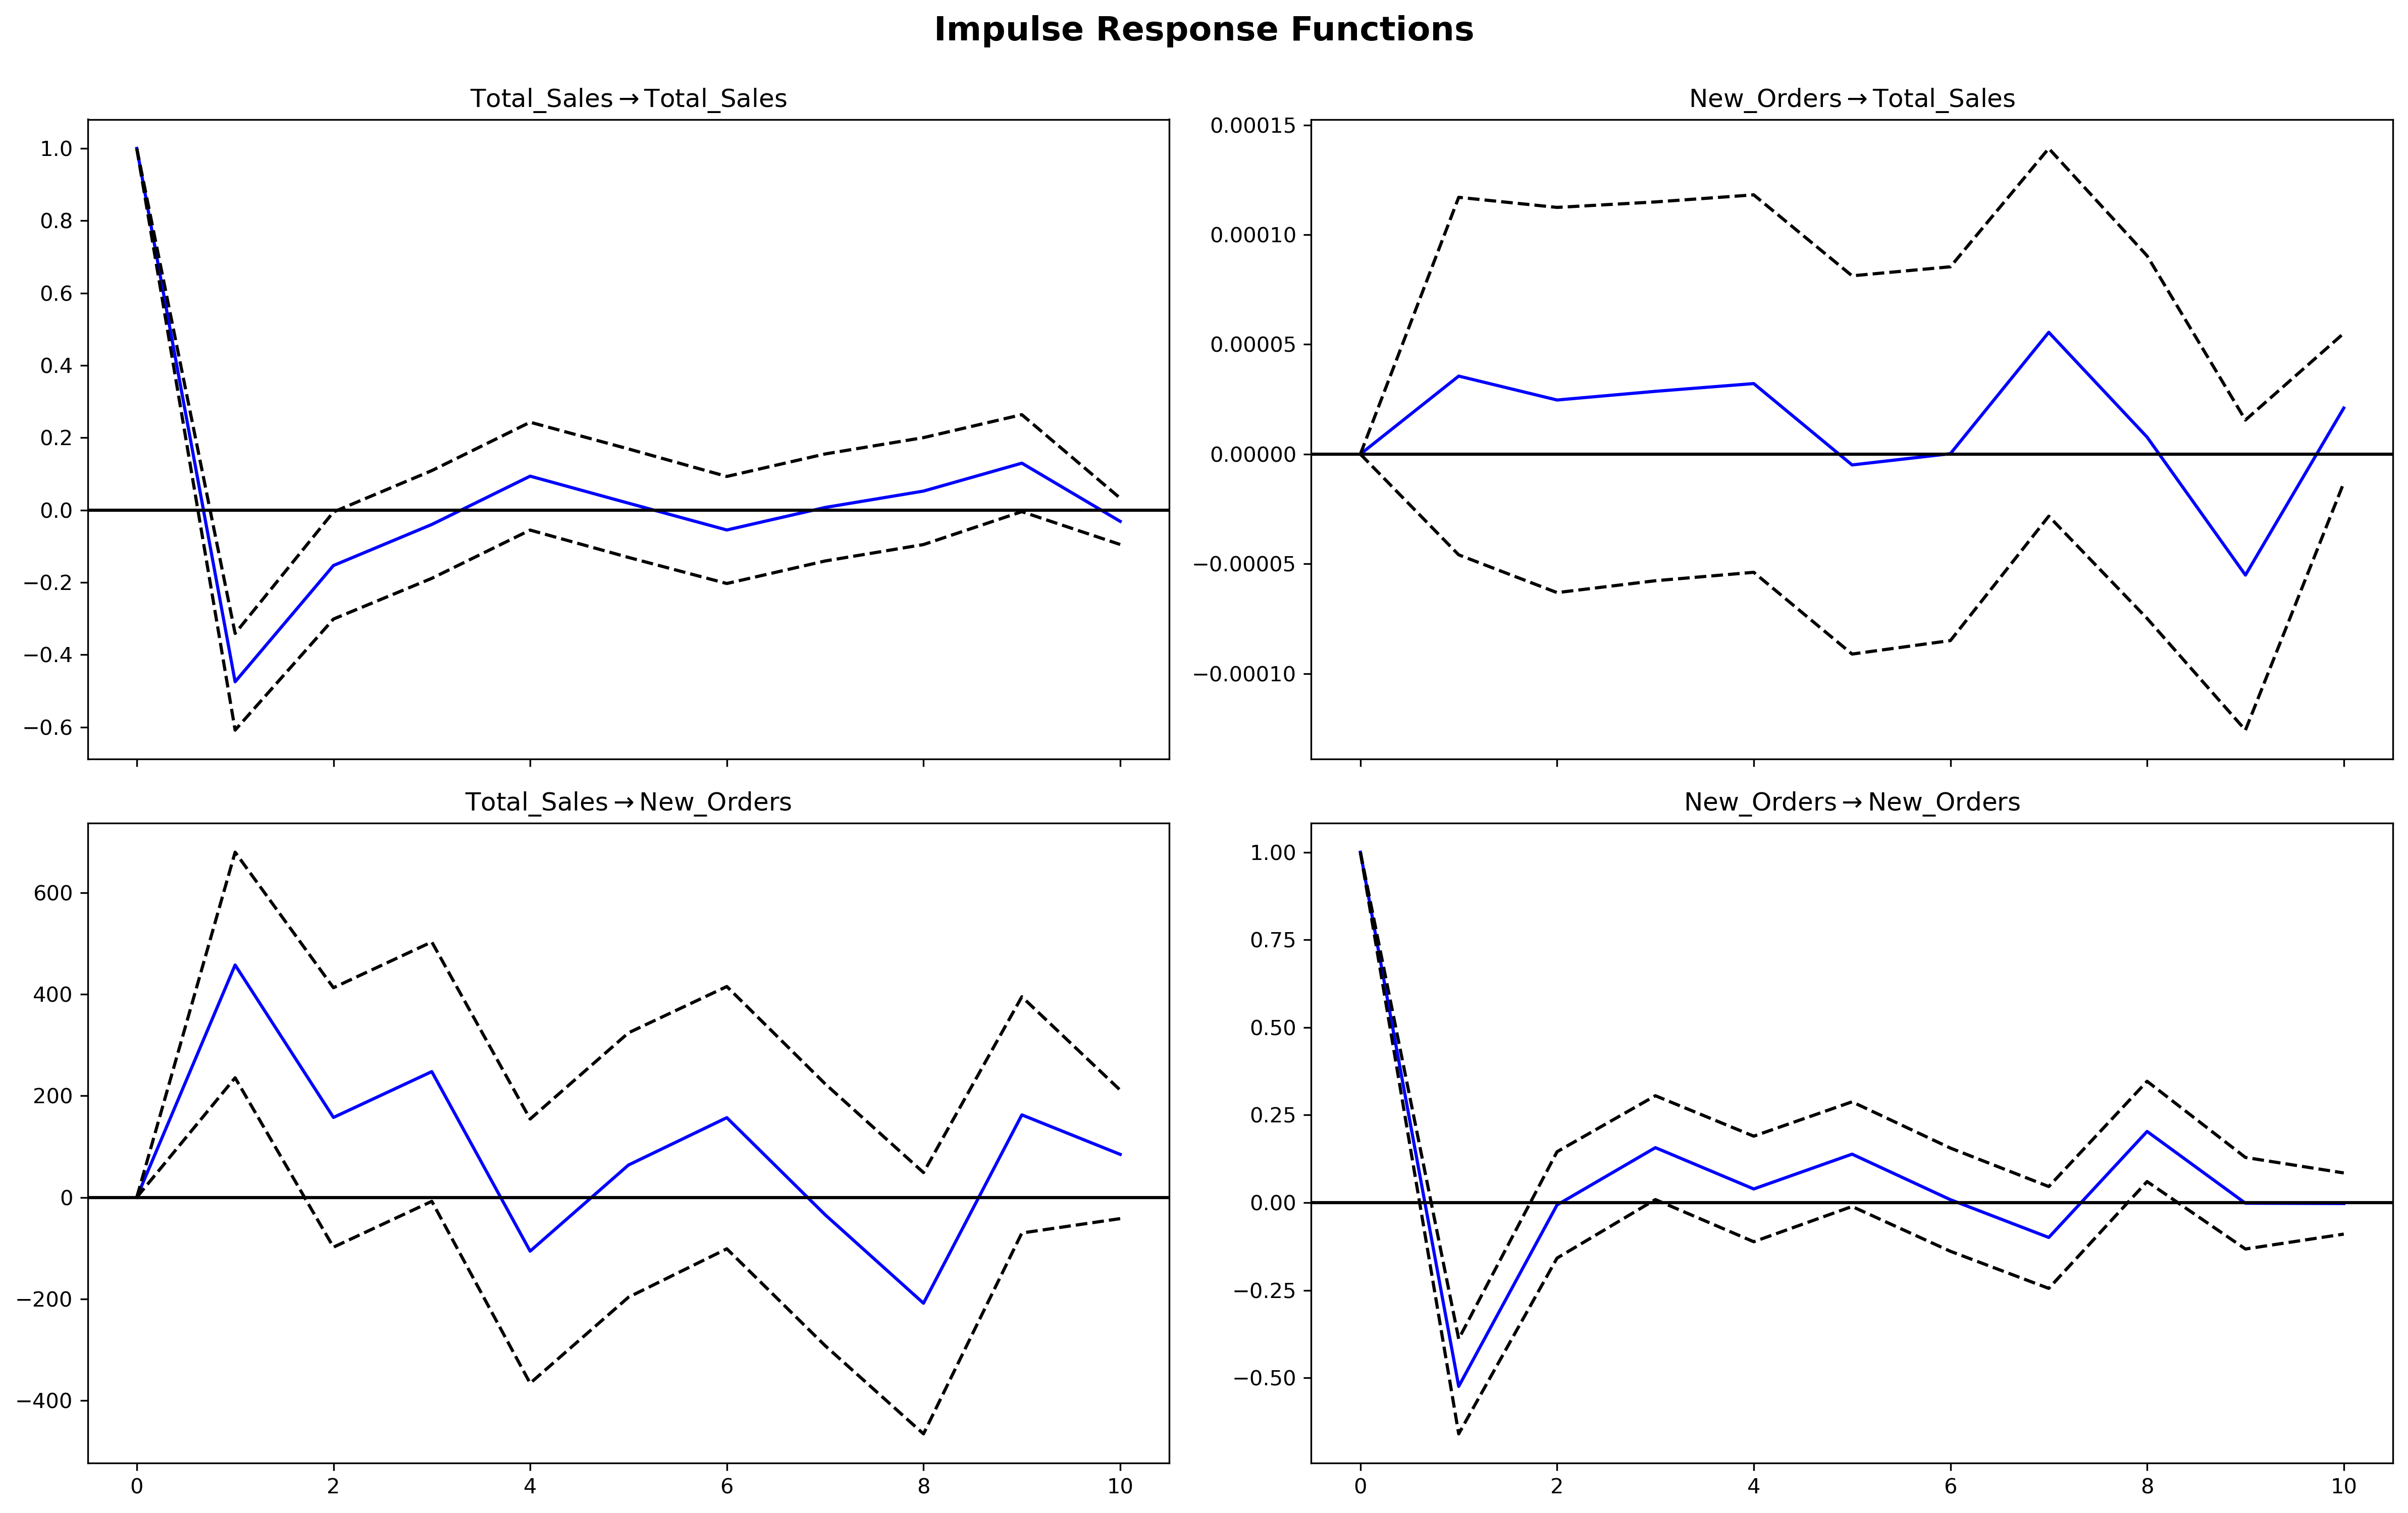
\includegraphics[width=0.65\textwidth]{outputs/impulse_response.png}
    \caption{Impulse Response Functions showing dynamic relationships between variables.}
\end{figure}

\begin{figure}[H]
    \centering
    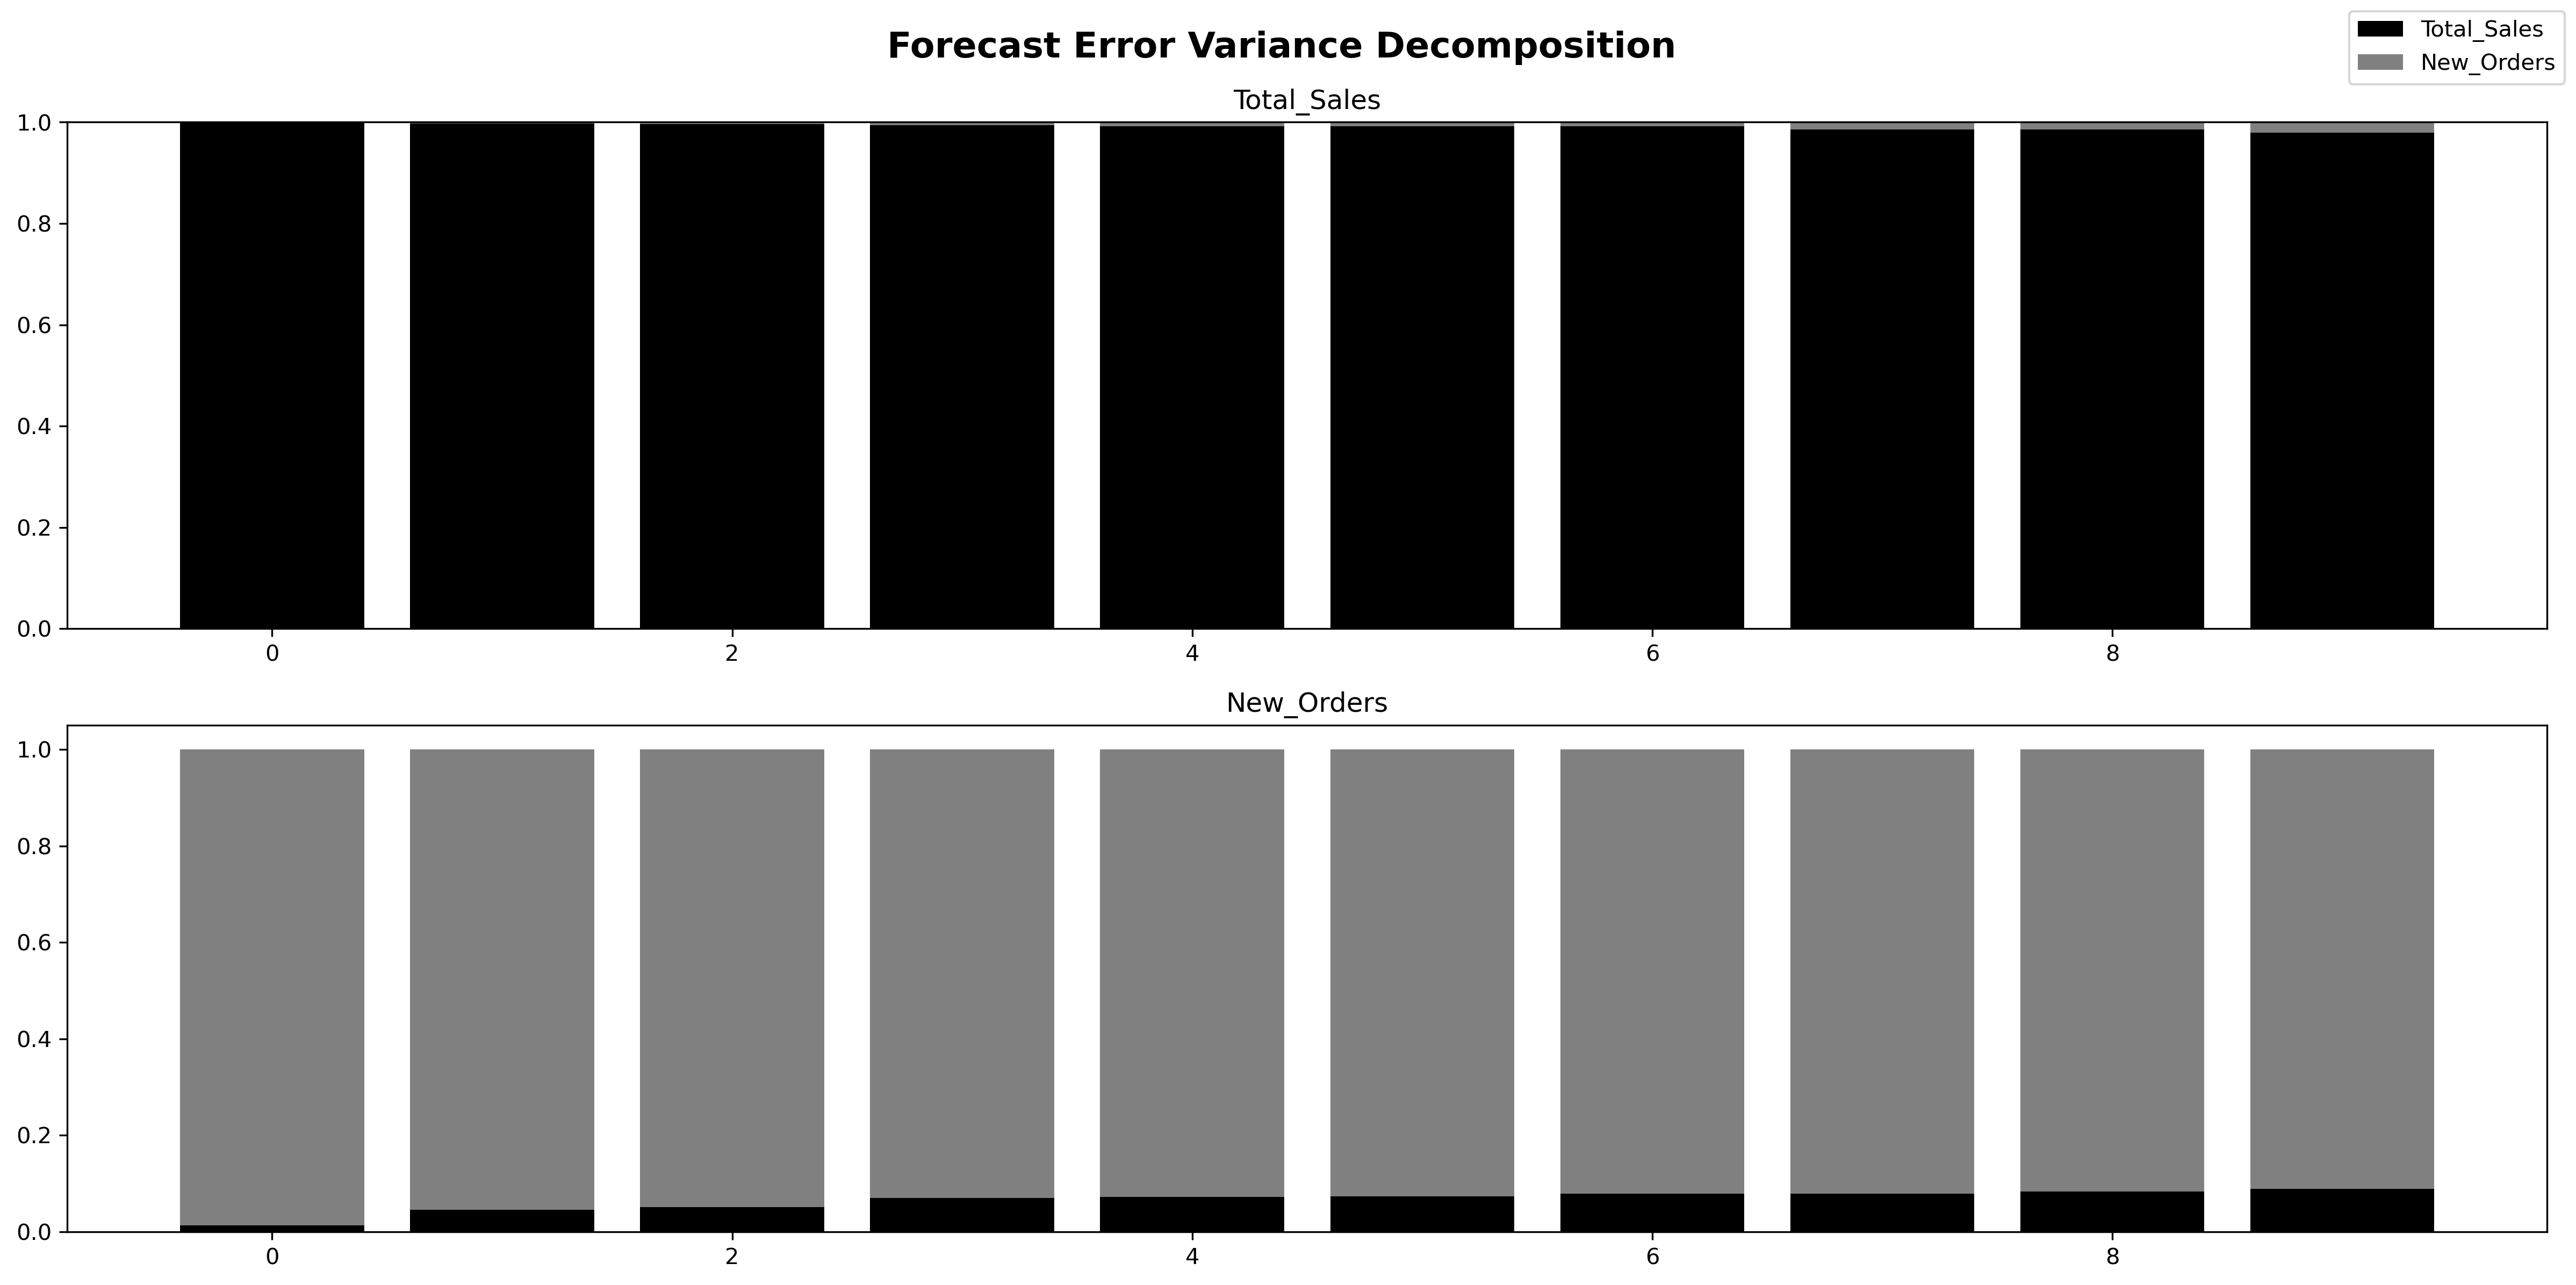
\includegraphics[width=0.65\textwidth]{outputs/fevd.png}
    \caption{Forecast Error Variance Decomposition over time horizon.}
\end{figure}

\section*{\textbf{Appendix B: Team Contributions}}
\addcontentsline{toc}{section}{Appendix B: Team Contributions}

\textbf{Team Member 1 - [Name]:} Conducted exploratory data analysis, stationarity testing (ADF, KPSS), seasonal decomposition, and created EDA visualizations. Developed ARIMA and SARIMA models, performed ACF/PACF analysis, conducted model selection using AIC/BIC, and generated forecast plots. Implemented VAR analysis, conducted Granger causality tests, and performed impulse response and FEVD analysis. Contribution: 50\%.

\textbf{Team Member 2 - [Name]:} Analyzed multivariate relationships and interpreted VAR results. Developed machine learning models (XGBoost, LightGBM), engineered temporal features, performed hyperparameter tuning, and conducted comprehensive model comparison. Performed literature review, wrote final report, created all documentation, and compiled results. Contribution: 50\%.

Both team members contributed equally to analysis plan development, results interpretation, report writing, and code review. Both team members contributed at least 80\% of expected work.

\section*{\textbf{Appendix C: Code Availability}}
\addcontentsline{toc}{section}{Appendix C: Code Availability}

All analysis code is available in the following files:
\begin{itemize}
    \item \texttt{Vehicle\_Analysis\_Complete.py} -- EDA, stationarity testing, seasonal decomposition
    \item \texttt{ACF\_PACF\_Analysis.py} -- Model identification and ACF/PACF plots
    \item \texttt{ARIMA\_SARIMA\_Modeling.py} -- ARIMA and SARIMA model implementation
    \item \texttt{VAR\_Analysis.py} -- VAR modeling, Granger causality, IRF, and FEVD
    \item \texttt{ML\_GradientBoosting\_Analysis.py} -- XGBoost and LightGBM implementation
    \item \texttt{run\_all\_analyses.py} -- Master script to execute all analyses
    \item \texttt{Vehicle\_Data\_Analysis.ipynb} -- Jupyter notebook with interactive analysis
\end{itemize}

All code is well-documented with inline comments and follows PEP 8 style guidelines.

\end{document}
